\documentclass{article}

\usepackage[OT1]{fontenc}
\usepackage{mathpazo}
\usepackage[italian]{babel}

%math
\usepackage{amsmath}
\usepackage{amssymb}
\usepackage{amsfonts}
\usepackage[utf8]{inputenc}
\usepackage{cancel}
\usepackage{listing}
\usepackage{listingsutf8}
\usepackage{listings}
%table
\usepackage{booktabs} % for better looking tables
\usepackage{siunitx}  % for units of measure and data in tables
    \usepackage{array}
    \usepackage{multirow}
    \usepackage{hhline,booktabs,amsmath}
    \usepackage{makecell}

%Graphics&Float
\usepackage{graphicx}
\usepackage{float}
\usepackage{chngcntr}
\counterwithin{figure}{section}
%
%Hypelinks
\usepackage{hyperref}
\hypersetup{
    colorlinks,
    citecolor=black,
    filecolor=black,
    linkcolor=black,
    urlcolor=black
}

% TIKZ
\usepackage{tikz}
\usetikzlibrary{shapes.geometric, arrows}
\tikzstyle{arrow} = [thick,->,>=stealth]
\tikzstyle{startstop} = [rectangle, rounded corners, minimum width=3cm, minimum height=1cm,text centered, draw=black, fill=red!30]
\tikzstyle{io} = [trapezium, trapezium left angle=70, trapezium right angle=110, minimum width=3cm, minimum height=1cm, text centered, draw=black, fill=blue!30]
\tikzstyle{process} = [rectangle, minimum width=3cm, minimum height=1cm, text centered, draw=black, fill=orange!30]
\tikzstyle{decision} = [diamond, minimum width=3cm, minimum height=1cm, text centered, draw=black, fill=green!30]

%Algorithm
\usepackage[]{algorithm2e}

\title{\textbf{Informatica Teorica}}
\author{Manuel Pagliuca}

\begin{document}
\maketitle
\pagebreak
\tableofcontents
\pagebreak
\newpage
\section{Introduzione}
Nei corsi di informatica applicata come quelli di: Sistemi Operativi, Basi di dati, ecc... l'oggetto di studio è definito dal corso, e l'informatica è lo strumento per studiare questo oggetto.

Nel corso di informatica teorica l'oggetto di studio è l'informatica stessa, si studiano i fondamenti dell'informatica (come un corso di sistemi operativi effettua uno studio sui fondamenti dei sistemi operativi).

Per eseguire lo studio di questa disciplina ci si pone le due domande fondamentali nei confronti dell'informatica \textit{cosa} e \textit{come}.
\subsection{Cosa studia l'informatica?}
L'informatica è una disciplina che studia l'informazione e l'elaborazione automatica mediante sistemi di calcolo che eseguono programmi.

Ma sappiamo che tutti i problemi sono risolubili per via automatica, e questo porta proprio alla nostra domanda, quali problemi sono in grado di risolvere \textit{automaticamente}?

Ciò che studia il \textit{cosa} dell'informatica si chiama \textbf{teoria della calcolabilità}, mostreremo nelle successive lezioni che non è una domanda cosi facile da rispondere, poichè esistono delle cose che non sono calcolabili. Quindi dato che non ci sono cose calcolabili, la teoria della calcolabilità si domanda \textit{che cosa è calcolabile?}.
\newline
Nella teoria della calcolabilità vogliamo una risposta generale, non cerchiamo dei casi particolari per dire questo è calcolabile o meno, esistono delle proprietà che accomunano tutto ciò che è calcolabile ? La risposta è si, la nozione di calcolabilità è denotabile attraverso la matematica e quindi posso affrontare l'insieme di cose fattibili dell'informatica con gli strumenti della matematica.
\subsection{Come l'informatica risolve i problemi?}
La branca dell'informatica che si chiama \textbf{teoria della complessità} risponde alla domanda \textit{come è risolubile questo problema ?}. Essa studia la quantità di risorse computazionali richieste dalla \textit{soluzione automatica} dei problemi. Una \textit{risorsa computazionale} è qualsiasi cosa venga sprecata per l'esecuzione dei programmi:

Le principali risorse su cui ci concentreremo sono il \textbf{tempo} e \textbf{spazio di memoria}, dovremo quindi dare una definizione rigorosa di queste risorse computazionali. Successivamente si potrà porre delle domande ovvie : \textit{quale è la classe di problemi che vengono risolti efficientemente in termini di tempo e di memoria ?}. Notare che nella teoria della complessità non si parla solo di \textbf{risolubilità} (come nella teoria della calcolabilità) ma anche dell'\textbf{efficienza} con cui risolvo questo problema.
\newline
Esistono problemi che si trovano in una zona grigia, che non sappiamo se hanno una risoluzione efficiente, ma sono problemi molto importanti, nessuno è riuscito a dimostrare se avranno soluzioni efficienti ma nemmeno il contrario, ovvero nessuno è riuscito a dimostrare che saranno risolubili efficientemente. Questa classe di problemi è la classe di problemi NP, vedremo poi di cosa si tratta.
\section{Syllabus}
\begin{itemize}
    \item Teoria della calcolabilità: individuare la qualità della calcolabilità dei problemi, quali sono le categorie di problemi calcolabili e distinguerla da quella dei problemi non calcolabili.
    \item Teoria della complessità: studio quantitativo dei problemi, dopo aver delimitato il confini di ciò che è calcolabile cercare un sotto insieme di problemi \textbf{efficientemente calcolabili}.
\end{itemize}

\pagebreak
\section{Il nostro linguaggio: la matematica}
\subsection{Funzione}
Una funzione dall'insieme $A$ all'insieme $B$ è una \textbf{legge}, che chiamiamo solitamente $f$, che spiega come associare ad ogni elemento di $A$ un elemento di $B$.
\newline

Dal punto di vista formale l'espressione della funzione viene definita \textbf{globalmente}:
$$f:A\rightarrow B$$
Dove $A$ viene chiamato \textbf{dominio} e $B$ \textbf{codominio}, questa notazione dice che ogni elemento del dominio è associato attraverso una legge $f$ ad un elemento del codominio. Esiste anche uan notazione che permette di stabilire localmente l'operato della funzione, essa rappresenta l'operato della legge $f$ sull'elemento $a$ che porta all'elemento $b$.
$$a \xrightarrow[\text{}]{\text{f}} b$$
\newline
La notazione comunemente più utilizzata (in particolare nei libri di testo, ma anche nei corsi di matematica), è la seguente:
$$f(a)=b$$
Solitamente $b$ è l'\textbf{immagine} di $a$ secondo $f$, e meno usualmente si dice che $a$ è la \textbf{controimmagine} di $b$ (sempre secondo $f$).
\newline
\newline
Per esempio:
$$f:\mathbb{N} \rightarrow \mathbb{N}$$
Dove $\mathbb{N}$ è l'insieme dei numberi naturali ${0,1,2,3,...}$, e per utilizzi futuri denotiamo con $\mathbb{N}^+$ l'insieme dei numeri naturali positivi (zero escluso) ${1,2,3,4,...}$.
\newline
Ora vediamo la specifica della funzione $f$
$$f(n)=\lfloor \sqrtsign{n}\rfloor$$
Considerando $n=5$ l'immagine di quest'ultima sarà $f(5)=\rfloor\sqrt{5}\lfloor=2$.
\newline
Quindi possiamo dedurre che per più elementi del dominio una \textbf{funzione} effettua un mapping ad uno ed un solo valore del codominio (nel caso in cui un valore del dominio venga mappato a più valori del codominio allora si parla di relazione, ma non più di funzione).
\subsection{Classi di funzioni}
\subsubsection{Funzioni iniettive}

Una funzione è \textbf{iniettiva} se e solo se elementi diversi del dominio vengono mappati in elementi diversi del codominio.
$$f:A\rightarrow B\text{ è iniettiva sse } \forall a_1,a_2\in A \text{ dove } a_1\neq a_2 \implies f(a_1)\neq f(a_2)$$
\newline
\textit{Esempio 1}
$$f(n)=\lfloor\sqrt(n)\rfloor$$
Abbiamo visto precedentemente che questa funzione non è iniettiva, perché avviene un mapping per più elementi del dominio ad un unico elemento del codominio.
\newline
\newline
\textit{Esempio 2}
$$f(n)=[n]_2$$
Questa funzione è fortemente non iniettiva, le due metà dell'insieme dei numeri naturali vengono mappate solamente su due numeri $f(2k)=0$ e $f(2k+1)=1$.
\newline
\newline
\textit{Esempio 3}
$$f(n)=n^2$$
Questa è una funzione iniettiva, poiché ad ogni controimmagine corrisponde una immagine distinta.

\subsubsection{Funzioni suriettive}
Una funzione è suriettiva quando tutti gli elementi del codominio hanno una corrispondenza con un elemento del dominio.
$$f:A\implies B\text{ sse } \forall b\in B, \exists a \in A : f(a)=b$$
\noindent
\textit{Esempio 1}
\newline
$f(n)=\lfloor\sqrt{n}\rfloor$ è suriettiva, questo perchè $\forall m\in \mathbb{N}, m=\lfloor\sqrt{m^2}\rfloor=f(m^2)$. Sostanzialmente, posso tornare con facilità al dominio perchè mi basta elevare al quadrato l'immagine, e questo è fattibile per tutto l'insieme dei numeri naturali.
\noindent
\newline
\linebreak
\textit{Esempio 2}
\newline
$f(n)=[n]_2$ non è una funzione suriettiva, questo perchè per esempio $3$ non è immagine di niente rispetto a $f$ (il codominio è tutto $\mathbb{n}$).

\subsection{Insieme immagine di una funzione}
$$Im_f={b\in B:\exists a,f(a)=b}={f(a):a\in A}$$

Data $f$ definitiamo l'\textbf{insieme immagine di $f$} come gli elementi del codominio $\in B$ che sono immagine di un elemento del dominio $A$.
\newline
La relazione tra questo insieme $Im_f$ ed il codominio stesso di $f$ quale è $B$, consiste in:
$$Im_f\subseteq B$$
Allora possiamo dire che una funzione è suriettiva quando:
$$Im_f=B$$
\newline
\textit{Esempi}
$$Im_{\lfloor\sqrt{n}\rfloor}=\mathbb{N}\implies f(n)=\lfloor\sqrt{n}\rfloor \text{ è suriettiva}$$
$$Im_{[n]_2}={0,1}\subseteq \mathbb{N} \implies f(n)=[n]_2 \text{ non è suriettiva}$$

\subsection{Funzioni biettive}
Una funzione si dice biettiva quando è sia suriettiva che iniettiva, devono valere entrambe le due condizioni (questo due condizioni è possibile fonderle in un unica condizione).
$$f:A\rightarrow B \textbf{ sse }$$
$$\forall a_1,a_2 \in A, a_1\neq a_2 \implies f(a_1)\neq f(a_2) \land \forall b\in B, \exists a\in A:f(a)=b$$
Che converge in un unica definizione:
$$\forall b \in B,\exists !a\in A : f(a)=b$$
Per esempio: $f(n)=n$, oppure considerando gli insiemi dei numeri reali $f(x)=x^3$. Solo per questa tipologia di funzioni esiste il concetto di \textbf{funzione inversa}.

\subsection{Inversa di una funzione}
Data una funzione $f$ biettiva si definisce l'inversa come $f^{-1}$ la funzione tale che crei un mapping tra l'immagine del codominio rispetto alla controimmagine del dominio.
$$f:A\rightarrow B$$
$$f^{-1}:B\rightarrow A \text{ tale che } f^{-1}(b)=a \Longleftrightarrow (a)=b$$

Per esempio l'inversa di $f(n)$ è $f^{-1}=n$, oppure l'inversa di $f(x)=x^3$ è $f^{-1}=\sqrt[3]{x}$ (considerando l'insieme dei numeri reali).

\subsection{Composizione di funzioni}
Date due funzioni $f:A\rightarrow B$ e $g:B\rightarrow C$, notiamo che queste funzioni hanno una caratteristica in comune, ovvero che il codominio di una è il dominio dell'altra.
Definiamo la composizione di funzione $g\circ f:A\rightarrow C$ come la funzione che va da dal dominio di $f$ al codominio di $g$, definita come $g(f(a))$.
$$g\circ f=g(f(a))$$

Per esempio $f(n)=n+1 \text{ e } g(n)=n^2$:
\begin{itemize}
    \item $f \text{ composto } g: g\circ f(n)=(n+1)^2$
    \item $g \text{ composto } f: f\circ g(n)=n^2+1$
\end{itemize}

N.B. L'operazione di composizione restituisce una funzione, e l'operatore $\circ$ non è commutativo, però quando dominio e codominio lo permettono è \textbf{associativo}: $(f\circ g)\circ h=f\circ (g \circ h)$.

\subsubsection{Funzione identità}
La funzione identità sull'insieme $A$ è una funzione che effettua un mappaggio ricorsivo sullo stesso elemento.
$$i_A:A\rightarrow A : i_A(a)=a\text{ }\forall a\in A$$
Per esempio la funzione identità sull'insieme $\mathbb{N}$ è $i_\mathbb{N}(n)=n$.

\subsubsection{Definizione alternativa di funzione inversa}
Data una funzione $f:A\rightarrow B$ biettiva, la sua inversa è l'unica funzione $f^{-1}:B\rightarrow A$ che soddisfa:
$$f^{-1}(b)=a \longleftrightarrow f(a)=b$$
$$oppure$$
$$f^{-1}\circ f=i_A \land f\circ f^{-1}=i_B$$

Infatti considerando $f^{-1}\circ f(x) = \sqrt[3]{x^3}=x=i_\mathbb{N}(x)$ e $f\circ f^{-1}(x)=(\sqrt[3]{x})^3=x=i_\mathbb{N}(x)$

\subsubsection{Funzioni totali e parziali}
Considerando una funzione $f:A\rightarrow B$ essa è una legge che ad \textbf{ogni} elemento di $A$ si associa
un elemento di $B$, questo significa che ogni immagine $f(a)$ è definita per ogni elemento $a\in A$. Esiste
un apposita notazione:
$$f(a)\downarrow \forall a\in A$$

Una funzione di questo tipo viene chiamata \textbf{totale} poiché risulta definita sulla totalità del suo dominio.

Certe funzioni potrebbero \textit{non essere definita} per quale che elemento di $a\in A$, e quindi non avere delle immagini corrispondenti, la notazione:
$$f(a)\uparrow$$
Ovvero, che per un elemento $a$ non esiste immagine nell'insieme $B$ tramite la funzione $f$.

Consideriamo il seguente esempio:
$$f:\mathbb{N}\rightarrow\mathbb{N}$$
$$f(n)=\lfloor\frac{1}{n}\rfloor \text{ non è definita su } n=0\implies f(0)\uparrow \forall n\in\mathbb{N}\setminus{0}, f(n)\downarrow$$

Una funzione viene definita \textbf{parziale} se a \textit{qualche} elemento di $A$ si associa un elemento di $B$. Si amplia un nuovo concetto che è quello del \textbf{dominio} (o campo di esistenza) della funzione,
ovvero quell'insieme costituito da tutti gli elementi di $A$ tali per cui è definita una immagine appartenente a $B$.
$$Dom_f=\left\{a\in A : f(a)\downarrow \right\}\subseteq A$$

Allora vale precisare le due seguenti regole:
$$Dom_f\nsubseteq A\implies f\text{ parziale}$$
$$Dom_f\equiv A\implies f \text{ totale}$$

Alcuni esempi:
$$f(n)=\left\{\frac{1}{n}+\frac{1}{(n-1)(n-2)}\implies Dom_f=\mathbb{N}\setminus\{0,1,2\right\}$$
$$f(n)=\lfloor\log{n}\rfloor\implies Dom_f=\mathbb{N}\setminus\{0\}$$
$$f(n)=\lfloor\sqrt{-n} \implies Dom_f=\{0\}$$
\subsubsection{Totalizzazione di una funzione parziale}
Teniamo conto di una cosa, possiamo convenzionalmente rendere totale una funzione parziale, basta estendere
il codominio con un \textbf{simbolo convenzionale} $\bot$ che buttiamo fuori tutte le volte che la funzione non è definita.
$$f:A\rightarrow B\text{ parziale } \implies \widetilde{f}:A\rightarrow B\cap\{\bot\}$$
La totalizzazione di $f$ viene raggiunta con l'aggiunta di questo simbolo.
\[
    \widetilde{f}(a) =
    \begin{cases}
        f(a) & \quad\text{se }a\in Dom_f \\
        \bot & \quad\text{altrimenti}    \\
    \end{cases}
\]
Quindi per i punti dove il campo di esistenza non è definito verrà restituito $\bot$, per convenzione
quando una funzione parziale viene totalizzata ovvero $B\cap\bot$ possiamo utilizzare la seguente
notazione $B_{\bot}$.

\subsubsection{Prodotto cartesiano}
$$A\times B=\{(a,b):a\in A \land b\in B\}$$
Il \textbf{prodotto cartesiano} di due insiemi è l'insieme di coppie dove il primo elemento della coppia appartiene al primo insieme, ed il secondo elemento della coppia appartiene al secondo insieme.

Il prodotto cartesiano è un'operazione che non commuta.
$$A\times B \neq B\times A$$
Ovviamente l'unico caso dove un prodotto cartesiano è commutativo è quando $A\equiv B$.
Il prodotto cartesiano può essere esteso al prodotto di ennuple di più insiemi cartesiani,
dove questa volta il risultato è costituito da un insieme ordinato (non più di coppie) delle ennuple
rispettive agli insiemi di provenienza:
$$A_1\times A_2 \times ... \times A_n=\{(a_1,a_2,...,a_n):a_i\in A_i$$

Associato alla definizione di prodotto cartesiano abbiamo anche quella di \textbf{proiettore i'esimo},
essa è una funzione che agisce su un prodotto cartesiano. Ha come dominio l'insieme i-esimo di questo prodotto data una tupla del prodotto cartesiano non fa altro che estrapolare la componente i-esima di quella tupla (\textit{destruttura la tupla}).
$$\pi_i:A_1\times ...\times A_n\rightarrow A_i$$
$$\pi_i(a_1,...,a_n)=a_i$$
Utilizzeremo la seguente notazione esponenziale per calcolare il prodotto cartesiano di un insieme cartesiano
con se stesso:
$$A_1\times A_2\times A_3 ... \times A_n = A^n$$

Alcuni esempi:

$$C=\{(x,y)\in\mathbb{R}^2 : x^2+y_2=1\}\implies \text{ punti che si trovano lungo la circonferenza}$$
$$I=\{(x,y)\in\mathbb{R}^2 : x^2+y_2<1\}\implies \text{ punti che si trovano all'interno della circonferenza}$$
$$E=\{(x,y)\in\mathbb{R}^2 : x^2+y_2>1\}\implies \text{ punti che si trovano all'esterno della circonferenza}$$

$$C\cap I\cap E = \mathbb{R}^2$$

\subsubsection{Insieme di funzioni}
L'insieme delle funzioni che vanno dall'insieme $A$ a $B$ viene indicato con:
$$B^A=\{f:A\rightarrow B\} = \text{ insieme delle funzioni da } A \text{ a } B$$

L'insieme delle funzioni \textit{parziali} che vanno da $A$ a $B$:
$$B_{\bot}^A =\{f:A\rightarrow B_{\bot}\}=\text{ insieme delle funzioni parziali che va da A a B}$$

\subsubsection{Funzione di valutazione}
Dati due insiemi $A,B$ e $B_{\bot}^A$ si definisce una funzione di valutazione come:
$$\omega : B_{\bot}^A\times A \rightarrow B \text{ con } \omega (f,a)=f(a)$$
Essa è una funzione che valuta il punto del codominio $A$ in termini di $B$, ovvero restituisce un
$f(a)$, quindi il suo compito è strettamente quello di valutare.

\begin{itemize}
    \item Tenendo fisso $a$ e facendo variare $f$, è come se $a$ fosse un \textit{benchmark}
          su cui testiamo una serie di funzioni.
    \item Tenendo fisso $f$ e facendo variare $a$ ottengo il grafico di $f$.
\end{itemize}

\subsection{Modellare teoricamente un sistema di calcolo}
Un sistema di calcolo è architettato come un architettura di Von Neumann, è un sistema che dato
in input un \textit{dato} $x$ ed un \textit{programma} $P$. L'output può essere indicato con $y$ quando è definito,
mentre con $\bot$ quando va in \textit{loop}.

\begin{figure}[H]
    \centering
    \begin{tikzpicture}[node distance=2cm]
        \node (dati)[
            minimum width=1cm,
            minimum height=1cm] at (0,1) {$x$};
        \node (prog)[
            minimum width=1cm,
            minimum height=1cm] at (2,1) {$P$};
        \node (model)[draw,
            minimum width=2cm,
            minimum height=1cm] at (1,-1) {$\mathcal{C}$};
        \draw [arrow] (dati) -- (model);
        \draw [arrow] (prog) -- (model);
        \node (output)[
            minimum width=1cm,
            minimum height=1cm] at (1,-3) {$y$ o $\bot$};
        \draw [arrow] (model) -- (output);
    \end{tikzpicture}
\end{figure}

$P\in PROG$: Un programma è una \textbf{sequenza di regole} scritte in un certo linguaggio
che prende un input e lo trasforma in un output (o in un loop).
Essenzialmente un programma è la definizione di una funzione scritta a mano, esso
realizza una funzione che parte dai dati in input ed ottiene i dati in output.

$$P\in DATI_{\bot}^DATI\text{ è una funzione in un linguaggio di programmazione.}$$

Quindi, ribadendo per l'ennesima volta un programma è la realizzazione di una
funzione, che va da un insieme di dati ad un altro.

Il sistema di calcolo in se prende in input dei dati ed una funzione (il programma),
che mi da un output, esso è definito come una \textbf{funzione di valutazione} $\mathcal{C}$.

$$\mathcal{C}:DATI_{\bot}^{DATI}\times DATI\rightarrow DATI_{\bot}$$
Quindi $\mathcal{C}$ è una funzione di valutazione, e $\mathcal{C}(P,x)$ è la funzione di valutazione
del programma $P$ sul dato $x$.

Per esempio, consideriamo il seguente programma:

\begin{algorithm}[H]
    \KwIn{$x$}
    \eIf{$\langle x\rangle_2==0$}{
        return $x$;
    }
    {
        \lWhile{$1<2$}{}
        return $1$;
    }

    \caption{Semantica di $P$}
\end{algorithm}

Voglio capire la semantica di questo programma è per capirlo voglio definire una
funzione che mi rappresenti il legame input-output rispetto ad un dato elemento.

Il programma prende in ingresso un numero intero, se il numero è pari restituisce
esattamente il numero intero, altrimenti entra in un loop (non termina).

$$\mathcal{C}(P,\_):\mathbb{N}\rightarrow\mathbb{N}_{\bot}$$
La \textbf{semantica} è la seguente :
\[
    \mathcal{C}(P,n) =
    \begin{cases}
        n    & \quad\text{se }n\text{ è pari} \\
        \bot & \quad\text{altrimenti}         \\
    \end{cases}
\]

\subsubsection{Potenza computazionale}
I sistemi di calcolo servono per calcolare le funzioni, ogni programma che immetto
nel mio sistema di calcolo mi viene calcolato. Indico con potenza computazionale
del mio sistema di calcolo è \textit{tutto quello che sa fare} il mio sistema di calcolo, o meglio,
tutte quelle funzioni che il mio sistema di calcolo può calcolare.

Tutte le funzioni che può calcolare il mio sistema di calcolo è un sottoinsieme
di tutte le funzioni immaginabili che possono andare da dati in dati. I programmi
in generale sono delle funzioni da dati in dati, quindi il mio sistema di calcolo
è ovvio che calcoli questo tipo di funzioni, è un sottoinsieme perchè non so quali
funzioni è in grado di risolvere il mio sistema di calcolo (e questa è la domanda
a \textit{cosa} a cui risponde l'informatica teorica).

$$F(\mathcal{C})=\{\mathcal{C}(P,\_):P\in PROG\}\subseteq DATI_{\bot}^{DATI}$$

Questo significa che esistono delle funzioni che non possono essere risolte dal mio
sistema di calcolo, e che quindi \textbf{non sono automatizzabili}.
$$F(\mathcal{C})\nsubseteq DATI_{\bot}^{DATI}$$
Sono presenti funzioni che l'informatica può risolvere e fare tutto.

$$F(\mathcal{C})=DATI_{\bot}^{DATI}$$

Quindi abbiamo ridotto il quesito \textit{che cosa sono in grado di fare i programmi},
ad un quesito matematico di inclusione propria ed impropria.
\subsubsection{Importanza del calcolo di funzione}
Calcolare una funzione significa risolvere problemi in \textit{generale}. Questo
perchè ad ogni problema posso associare una \textit{funzione soluzione}, non è altro che
quella funzione che ad un dato input associa una determinata \textit{soluzione}.
Per esempio, il \textit{problema del calcolo del determinante}:
\newline
DET:
\begin{algorithm}[H]
    \KwIn{$M\in \mathbb{R}^{n\times n}$}
    \KwOut{Determinante di $M$}
\end{algorithm}
La rispettiva funzione soluzione:
$$f_{DET}:\mathbb{N}^{n\times n}\rightarrow \mathbb{Z}$$
$$f_{DET}(M)=Det(M):$$
Vediamo che risolvere il dato problema consiste nel calcolare la funzione soluzione,
o risolvere il problema significa sostanzialmente avere un programma in grado
di risolvere quella funzione.

Find-Replace:
\begin{algorithm}[H]
    \KwIn{Testo, parola da cercare, parola da sostituire}
    \KwOut{Testo in cui ogni occorrenza della parola da cercare è sostituita dall'altra}
\end{algorithm}
La funzione soluzione:
$$f_{Find-Replace}:TESTI\times PAROLE\times PAROLE\rightarrow TESTI$$
$$f_{Find-Replace}(\text{La nostra vita,nostra,vostra})=\text{La vostra vita}$$

\subsubsection{Cardinalità degli insiemi - I°}
Siamo arrivati al primo punto fondamentale, il \textit{cosa} dell'informatica, ed
abbiamo visto che si concretizza nell'interrogarsi sulla relazione tra l'insieme della
potenza computazionale e quello di tutte le funzioni che vanno da dati in dati possibili.
$$F(\mathcal{C})\text{ ? }DATI_{\bot}^{DATI}$$

Per cercare di dare una dimostrazione sul carattere dell'inclusione, è molto utile
fare riferimento al concetto matematica di \textbf{cardinalità}.

Dato un insieme $A$, la sua cardinalità si indica con $|A|$. Intuitivamente che la cardinalità
di un insieme è il numero di elementi da cui è formato l'insieme. Questa idea intuitiva
è abbastanza corretta quando si ha a che fare con insiemi finiti (la cardinalità mi può
aiutare a capire quale insieme è più grande degli altri).

Purtroppo però quando tiriamo in ballo insiemi di cardinalità infinita, questo potrebbe
portare a conclusioni più complicate da elaborare. Si potrebbe \textit{erroneamente}
pensare $|\mathbb{N}|=\infty=|\mathbb{B}|$, ma questo sappiamo che
non è assolutamente vero, perchè l'insieme dei numeri reali è molto più fitto
di quello dei numeri interi.

Quindi dobbiamo aggiungere dei nuovi concetti, visto che \textit{"l'infinito di $\mathbb{R}$"} è
diverso da quello di $\mathbb{N}$. Il concetto da introdurre è quello di \textbf{relazione}.

\subsubsection{Relazione}
Consideriamo un insieme $A$, si definisce \textbf{relazione binaria} $R$ su $A$,
il sottoinsieme del prodotto cartesiano di $A$ su se stesso.
$$R\subseteq A^2$$
Gli elementi $a,b\in A$ stanno in una relazione $R$ se e solo se $(a,b)\in R$. Sono
presenti due notazioni infisse per denotare l'esistenza della relazione tra i due
elementi:
$$a\text{ R }b \text{ oppure } a\text{ \cancel{R} }b$$
Consideriamo per esempio la relazione $R$ come la relazione che agisce sui numeri naturali,
tale che un numero divida l'altro.
$$R\equiv \text{divide}: 3\text{ R }6, 5\text{ R }45, ...,3\text{ \cancel{R} }10$$
$$R=\{(a,b)\in\mathbb{N}^2:\langle b\rangle_a=0\}$$
Introduciamo anche il concetto di \textit{equivalenza in modulo} $k$, la quale mi
descrive una relazione del tipo:
$$a\equiv_k b \text{ sse } \langle a\rangle_k =\langle b\rangle_k$$
Per esempio: $5\equiv_2 7, 4\equiv_2 16,...$ (quando il resto dato dal divisore $k$ è
uguale su entrambi gli operandi).
\newline
Parliamo di \textbf{relazione di equivalenza} se e solo se soddisfa le seguenti
proprietà:
\begin{itemize}
    \item \textbf{Riflessiva}: $\forall a\in A, a\text{ R }a$
    \item \textbf{Simmetrica}: $\forall a,b\text{, } a\text{ R }b \Leftrightarrow b\text{ R }a$
    \item \textbf{Transitiva}: $\forall a,b,c\text{, }a\text{ R }b\land b\text{ R }c\implies a\text{ R }c$
\end{itemize}

Ora considerando le precedenti relazioni, vediamo che la relazione $R\equiv\textit{"divide"}$
non è una relazione di equivalenza:
\begin{itemize}
    \item È riflessiva.
    \item \textbf{Non è simmetrica}: $3\text{ R }6$ ma $6\text{ \cancel{R} }3$.
    \item È transitiva.
\end{itemize}
Mentre per la seconda relazione $\equiv_k$ possiamo dire che essa è una
relazione di equivalenza:
\begin{itemize}
    \item È riflessiva.
    \item È simmetrica, vengono valutati i modulo non direttamente gli operandi.
    \item è transitiva (per lo stesso motivo ancora).
\end{itemize}
Con una relazione di equivalenza è possibile effettua un \textbf{partizionamento
    delle classi di equivalenza}.
\subsubsection{Relazioni di equivalenza e partizioni}
Considerando una relazione di equivalenza $R\subseteq A^2$ induce una
\textbf{partizione} su $A$.
Le partizioni sono dei sottoinsiemi $A_1,A_2,A_3,...\subseteq A$ tali che:
\begin{itemize}
    \item $A_i\neq\emptyset$ (non sono vuoti).
    \item $i\neq j\implies A_i \cap A_j =\emptyset$ (non sono sovrapponibili).
    \item $\bigcup\limits_{i=1} A_i=A$ (la loro unione ricompone $A$).
\end{itemize}

Una \textbf{classe di equivalenza} di un elemento $a\in A$ è l'insieme di tutti
gli elementi che sono in relazione con $a$, notazione:
$$[a]_R=\{b\in A: a\text{ R }b\}$$
Si dimostra facilmente che :
\begin{itemize}
    \item Non esistono classi di equivalenza vuote, questo per via della proprietà
          \textit{riflessiva} delle relazioni di equivalenza.
    \item Se prendo due elementi diversi del dominio le classi di equivalenza relative
          o sono disgiunti o sono la stessa classe di equivalenza: $a,b\in A$ vale che
          $[a]_R\cap[b]_R=\emptyset$ o $[a]_r = [b]_R$.
    \item $\bigcup\limits_{a\in A}[a]_R=A$
\end{itemize}

Quindi la partizione indotta da una relazione di equivalenza non è altro che l'insieme
delle classi di equivalenza relative a quella relazione.
\newline
L'insieme delle classi di equivalenza di $R$ è la partizione indotta da $R$ su $A$.
\begin{figure}[H]
    \centering
    
\includegraphics[scale=0.4]{images/rel_equi_graph.png}
    \caption{Insieme $A$ partizionato}
\end{figure}

L'insieme $A$ partizionato rispetto alla relazione $R$ è detto \textbf{insieme quoziente}:
$$A / R$$

Quindi il quoziente di $A$ rispetto a $R$ è lo \textit{"spezzettamento"} di $A$ in classi
di equivalenza.

Consideriamo il seguente esempio di insieme quoziente, consideriamo la relazione di equivalenza $\equiv_4\subseteq\mathbb{N}$.
\textit{Quali classi di equivalenza ammette questa relazione ?}
$$[0]_4={4k}\text{ tutti i multipli di 4 hanno lo stesso resto di 1}$$
$$[1]_4={4k+1}\text{ tutti i multipli di 4 aumentati di 1 hanno lo stesso resto 1}$$
$$[2]_4={4k+2}; [3]_4={4k+3};...$$
\textit{Ne esistono altre ?} No, non esistono altre classi di equivalenza perché
ogni caso successivo a quelli \textit{"base"} si riconduce a quelli \textit{"base"}.
$$\langle n\rangle_2\in\{0,1,2,3\}$$
Voglio vedere se queste classi di equivalenza può rappresentare una partizione:
\begin{itemize}
    \item Nessuna classe è vuota.
    \item Sono mutuamente disgiunte, poiché se prendo un numero esso ricadrà
          solamente in una di queste classi di equivalenza.
    \item L'unione di queste $3$ classi di equivalenza restituisce l'insieme originale
          $\bigcup\limits_{i=0}^3 [i]_4=\mathbb{N}$.
\end{itemize}
\begin{figure}[H]
    \centering
    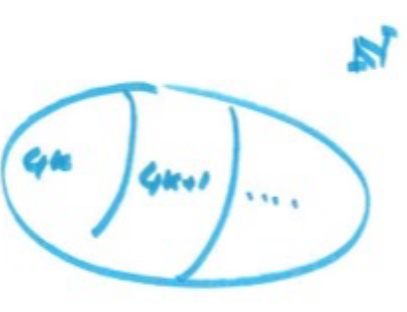
\includegraphics[scale=0.4]{images/rel_equi_quot.png}
    \caption{Insieme quoziente di $\equiv_4$}
\end{figure}

$\{[i]_4 : 0\leq i\leq 3\}$ è una partizione di $\mathbb{N}$ indotta dalla relazione
$\equiv_4$, tale per cui mi dia il rispettivo insieme quoziente (a volte impropriamente
chiamato $\mathbb{Z}_4$):
$$N / \equiv_4 \text{ }=\{[i]_4 : 0\leq i\leq 3\}=\mathbb{Z}_4$$

Adesso abbiamo in mano gli strumenti per definire in maniera molto più fine il concetto
di cardinalità.

\subsubsection{Cardinalità degli insiemi - II°}
Sia $\mathcal{U}$ (insieme universo) la classe di tutti gli insiemi,
definiamo la relazione $\sim\subseteq\mathcal{U}^2$ detta relazione
di \textit{equi numerosità} (hanno la stessa dimensione numerica), tra le coppie degli insiemi, se e solo se esiste
una \textbf{biezione} tra $A$ e $B$ (ovvero, se riesco ad esibire una funzione
iniettiva e suriettiva che va da $A$ in $B$).

Questa relazione tra insiemi è una relazione di equivalenza, poiché:
\begin{itemize}
    \item $\sim$ è riflessiva, se utilizzo la funzione identità $i_A$.
    \item $\sim$ è simmetrica, se esiste una biezione $A\rightarrow B$ allora
          esiste una biezione anche $B\rightarrow A$. Ovvero $A\sim B$ e $B\sim A$.
    \item $\sim$ è transitiva, se compongo funzioni biettive ottengo ancora una
          funzione biettiva.
\end{itemize}

Due insiemi che stanno in questa relazione vengono detti \textit{equi numerosi}. Ora
considerando l'insieme quoziente del nostro universo $\mathcal{U}$ rispetto alla
relazione di equi numerosità $\sim$ (quindi stesso numero di elementi in entrambi
i due insiemi), esso mi rappresenta il concetto di \textbf{cardinalità}
di un insieme.

\begin{figure}[H]
    \centering
    \includegraphics[scale=0.4]{images/insieme_quoziente_cardinalità.png}
    \caption{Insieme quoziente $\mathcal{U} / \sim$}
\end{figure}

Quindi spezzettando l'insieme $\mathcal{U}$ in classi di equivalenza
in questa classe di equivalenza ci sono tutti gli insiemi
che sono equi numerosi (seppur diversi).

Questo concetto permette di parlare in maniera molto precisa anche di
insiemi di cardinalità infinita.
Questi insiemi possono avere lo stesso numero
\newline
\newline
Per esempio, consideriamo $n\in\mathbb{N}^+$, si consideri l'insieme $J_n=\{1,2,,...,n\}$. Per questo
insieme è ovvio quale sia il concetto di cardinalità perchè è finito.

Allora diciamo che un insieme $A$ ha cardinalità \textbf{finita} se è equi
numeroso con $J_n$ (ovvero $A\sim J_n$) per un dato $n$ ed in quel caso scriviamo che $|A|=n$.

Quindi nella classe di equivalenza $J_1$ troviamo tutti gli insiemi con un
elemento, nella classe di equivalenza di $J_2$ troveremo tutti gli insiemi con due elementi, ecc.
\begin{figure}[H]
    \centering
    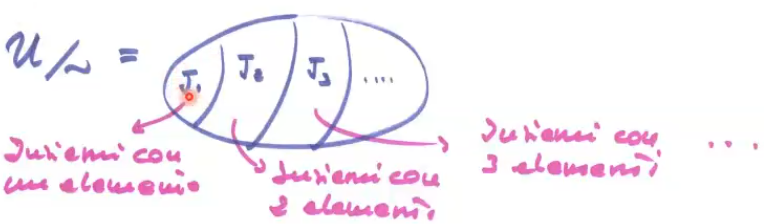
\includegraphics[scale=0.5]{images/U_insiemi_esemp_card2.png}
    \caption{Esempio $\mathcal{U}/\sim$ rispetto all'insieme $J_n$}
\end{figure}
Un insieme che non ha cardinalità si dice banalmente che ha cardinalità \textbf{infinità}. Fin qui abbiamo
parlato ancora di cardinalità finita, ma adesso faremo un esempio con cardinalità infinita.

\subsubsection{Insiemi numerabili}
$A$ si dice \textbf{numerabile} se è nella stessa classe di equivalenza dell'insieme dei numeri naturali
$\mathbb{N}$, ovvero se esiste una \textit{biezione} tra l'insieme $A$ e l'insieme $\mathbb{N}$.

Siccome stanno in relazione di equi numerosità
vuol dire che è presente una biezione fra i due elementi, quindi due elementi non possono collidere.

\begin{figure}[H]
    \centering
    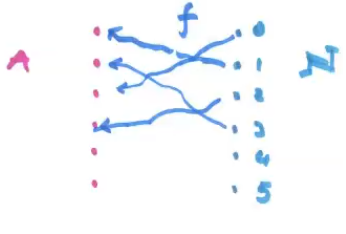
\includegraphics[scale=0.6]{images/A_numerabile_N.png}
    \caption{$A$ è un insieme numerabile}
\end{figure}

La presenza di questa biezione significa che come $A$ può essere \textbf{listato} con
$f(0),f(1),f(2),...$ su $\mathbb{N}$ senza perdere un elemento, anche l'insieme $\mathbb{N}$ può essere
listato a sua volta su $A$.

Alcuni esempi di insiemi numerabili:
\begin{itemize}
    \item I numeri pari $f(n)=2n$ , essi sembrerebbero la metà dei numeri naturali ma sono tanti quanto i numeri
          naturali perchè esiste questa biezione (vale anche per i dispari $f(n)=2n+1$).
    \item L'insieme $\mathbb{Z}$, possono essere presenti diverse funzioni, per esempio
          posso mappare i negativi sui numeri pari ed i positivi sui numeri dispari.
    \item L'insieme $\mathbb{Q}$, vedremo più avanti.
    \item L'insieme delle stringhe binarie che incominciano con $1$, ovvero $1\{0,1\}^*$,
          dove una funzione $f(n)=bin(n)$ è in grado di associare un numero naturale (utilizzando
          le potenze in posizione) ad una stringa binaria.
\end{itemize}

\subsection{Insiemi non numerabili}
Esistono degli insiemi che non sono listabili, dette in altre parole sono più fitti di $\mathbb{N}$,
è un altro tipo di categoria di infinito.
$$\mathbb{R}\text{ non è numerabile}$$
\paragraph{Dimostrazione}\mbox{}\\L'idea consiste nel dimostra per assurdo che non esiste una biezione
perchè sono presenti dei "buchi" tra le associazioni. Ordine della dimostrazione:
\begin{itemize}
    \item Dimostro che $\mathbb{R}\sim[0,1]$ (si dice che è \textit{isomorfo/equi numeroso} all'intervallo $[0,1]$),
          ovvero che è fitto quanto l'intervallo citato.
    \item Dimostro che $\mathbb{N}\nsim[0,1]$
    \item $\mathbb{R}\sim[0,1]\nsim\mathbb{N}\implies\mathbb{R}\nsim\mathbb{N}$
\end{itemize}

\paragraph{Dimostrazione $R\sim[0,1]$}\mbox{}\\ \noindent Significa riuscire a rappresentare una funzione
che mappa gli elementi tra i due insiemi in maniera che sia suriettiva ed iniettiva.

Prima di tutto abbiamo una retta cartesiana con un origine fissata e che copre tutti i numeri reali.
Pongo l'intervallo $[0,1]$ in modo che si trovi in corrispondenza del punto mediano della retta $0$,
successivamente prendo un compasso punto il centro nel mediano dell'intervallo e traccio la
semi circonferenza rispetto alla metà dell'intervallo.
\begin{figure}[H]
    \centering
    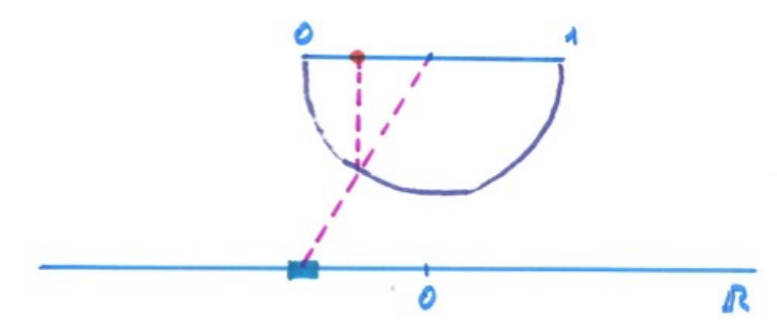
\includegraphics[scale=0.5]{images/dim_1.png}
    \caption{Dimostrazione  $R\sim[0,1]$}
\end{figure}

Gli elementi dell'insieme $\mathbb{R}$ vengono mappati tracciando una retta in direzione del punto
mediano di $[0,1]$, nel punto di intersezione si traccia la retta perpendicolare che interseca
l'intervallo ed in quel punto si trova il valore corrispondente. Si può fare lo stesso
in maniera opposta partendo da $[0,1]$, trovando l'intersezione si parte dal punto mediano
di quest'ultima e si attraversa l'intersezione toccando $\mathbb{R}$.

Questo dimostra che tutti i valori di $\mathbb{R}$ sono associabili
su $[0,1]$, quindi $\mathbb{R}\sim[0,1]$.

\paragraph{Dimostrazione $\mathbb{N}\nsim[0,1]$ (per diagonalizzazione)}\mbox{}\\Supponiamo per assurdo che $\mathbb{N}\sim[0,1]\implies[0,1]$,
ovvero che sia listabile (\textit{elencabile}) in maniera esaustiva così come lo è $\mathbb{N}$.
Siccome sto ipotizzando che sia elencabile, allora creo una lista di tutti gli elementi in $[0,1]$, i numeri
all'interno di questo numero seguono il formato "$0.$", quindi:
\[
    \begin{array}{ccccc}
        \underline{0.a_{11}} & 0.a_{12}             & 0.a_{13}             & 0.a_{14}             & ... \\
        0.a_{21}             & \underline{0.a_{22}} & 0.a_{23}             & 0.a_{24}             & ... \\
        0.a_{31}             & 0.a_{32}             & \underline{0.a_{33}} & 0.a_{34}             & ... \\
        0.a_{41}             & 0.a_{42}             & 0.a_{43}             & \underline{0.a_{44}} & ... \\
        ...                  & ...                  & ...                  & ...                  & ... \\
    \end{array}
\]
Se riesco a costruire un numero che non fa parte di questa lista infinita (elusivo alla biezione),
allora vuol dire che la lista non è elencabile, e quindi $[0,1]$ non è numerabile.

Per costruire questo numero elusivo che non si trova in nessuno di questi elementi della lista,
vado a guardare le cifre sulla \textit{diagonale}.\\Costruiamo il numero elusivo alla lista
$$0.c_1c_2c_3c_4$$
Tale che rispetti la seguente regola rispetto alla diagonale del elenco dei numeri $\in [0,1]$
\[
    c_i=
    \begin{cases}
        a_{ii} + 1\text{ se }a_{ii} < 9 \\
        a_{ii} - 1\text{ se }a_{ii} = 9 \\
    \end{cases}
\]
Ora usando questa regola non riuscirò mai a posizionare il mio nuovo numero
tra quelli elencati, questo perchè ovviamente cambio le cifre (il perché questo accade
probabilmente è collegato al fatto che $\mathbb{R}$ è più fitto di $\mathbb{N}$, proprio
quello che vogliamo dimostrare).
Il numero $0.c_1c_2...\in[0,1]$, ma non appartiene nelle liste poiché:
\begin{itemize}
    \item Differisce dal primo perché $c_1\neq a_{11}$
    \item Differisce dal secondo perché $c_2\neq a_{22}$
    \item Differisce da qualunque numero presente sulla diagonale
\end{itemize}
Quindi la lista non è esaustiva $\implies \mathbb{N}\nsim[0,1]$, significa che non cattura tutto l'intervallo $[0,1]$,
quindi non può esistere una biezione tra questo ed $\mathbb{N}$, ovvero $[0,1]$ \textbf{non è numerabile}.

\paragraph{Conclusione}\mbox{}\\
$$\mathbb{R}\sim[0,1]\nsim\implies\mathbb{R}\nsim\mathbb{N}$$
\begin{itemize}
    \item $\mathbb{R}$ non è numerabile.
    \item Esso è più \textit{"fitto"} di $\mathbb{N}$.
    \item Qualsiasi tentativo di listare anche solo un segmento non è esaustivo.
    \item $\mathbb{R}$ è un insieme \textbf{continuo}, e tutti gli insiemi equi numerosi
          $\mathbb{R}$ si dicono continui.
    \item Altri esempi di insiemi non numerabili:
\end{itemize}

\subsubsection{Insieme delle parti di $\mathbb{N}$}
Un altro insieme non numerabile è quello costituito dalla famiglia di sottoinsiemi possibili di $\mathbb{N}$,
quindi mettendo assieme uno dopo l'altro tutti i sottoinsiemi di differenti cardinalità (talvolta chiamato
\textbf{insieme potenza} o \textbf{booleano di} $\mathbb{N}$). Per esempio su un insieme $S=\{a,b,c\}$,
l'insieme delle parti è $\mathcal{P}(S)=\{\emptyset,\{a\},\{b\},\{c\},\{a,b\},\{a,c\},\{b,c\},S\}$.

$$\mathcal{P}(\mathbb{N})=2^{\mathbb{N}} = \{\text{sottoinsiemi di }\mathbb{N}\}\nsim\mathbb{N}$$
Anche questa dimostrazione avviene per diagonalizzazione, per assurdo suppongo che esista una
biezione che mi permetta di elencare tutti i sottoinsiemi di $\mathbb{N}$.

Posso rappresentare i sotto insiemi di $\mathbb{N}$ utilizzando un \textbf{vettore caratteristico}
$A\subseteq\mathbb{N}$, questo è un vettore dove metto il bit di appartenenza rispetto alla corrispondenza
dell'elemento.
\[
    \mathbb{N}\rightarrow
    \begin{array}{cccccccc}
        0 & 1 & 2 & 3 & 4 & 5 & 6 & ... \\
    \end{array}
\]
\[
    A\rightarrow
    \begin{array}{cccccccc}
        0 & 1 & 1 & 0 & 1 & 1 & 0 & ... \\
    \end{array}
\]
Allora se io suppongo per assurdo che $\mathcal{P}(\mathbb{N})\sim\mathbb{N}$, ovvero che è numerabile
rispetto all'insieme dei numeri naturali, allora posso elencare in maniera esaustiva i sotto insiemi
di $\mathbb{N}$, questo elencandone i vettori caratteristici.
\[
    \begin{array}{ccccc}
        \underline{0.b_{11}} & 0.b_{12}             & 0.b_{13}             & 0.b_{14}             & ... \\
        0.b_{21}             & \underline{0.b_{22}} & 0.b_{23}             & 0.b_{24}             & ... \\
        0.b_{31}             & 0.b_{32}             & \underline{0.b_{33}} & 0.b_{34}             & ... \\
        0.b_{41}             & 0.b_{42}             & 0.b_{43}             & \underline{0.b_{44}} & ... \\
        ...                  & ...                  & ...                  & ...                  & ... \\
    \end{array}
\]
Se riesco a costruire un sottoinsieme di $\mathbb{N}$ (vettore caratteristico) che non fa parte da di questa lista,
allora l'insieme delle parti non è un insieme numerabile poiché non è equi-numeroso con $\mathbb{N}$. Questo
è possibile procedendo per \textit{diagonalizzazione}, per esempio se considerassi il seguente vettore negato:
\[
    \begin{array}{ccccc}
        \overline{b_{01}} & \overline{b_{12}} & \overline{b_{23}} & \overline{b_{34}} & ... \\
    \end{array}
\]
riesco a constatare che esso non appartiene alla lista nonostante sia un sottoinsieme di $\mathbb{N}$
in quanto composto solo da valori booleani.

$$\mathcal{P}(\mathbb{N})\nsim\mathbb{N}$$

\subsubsection{Insieme $\mathbb{N}^{\mathbb{N}}$}
Consideriamo l'insieme di tutte le funzioni possibili funzioni che vanno da $\mathbb{N}$ in $\mathbb{N}$.
$$\mathbb{N}^{\mathbb{N}}=\{f:\mathbb{N}\rightarrow\mathbb{N}\}$$

Ipotizzando che $\mathbb{N}^{\mathbb{N}}\sim\mathbb{n}$, consideriamo la seguente tabella dove nella prima
colonna si trova l'elenco esaustivo di tutte le funzioni $\in\mathbb{N}$, e nelle colonne successive tutto
il dominio completo di $\mathbb{N}$. Significa che per ogni riga sara presente l'insieme dei valori che
fornisce il grafico di una funzione $f_i$.
\begin{center}
    \begin{tabular}{c|ccccc}
        \toprule
        Elenco delle funzioni di $\mathbb{N}$ & \textbf{0}           & \textbf{1}           & \textbf{2}           & \textbf{3}            & \textbf{...$\in\mathbb{N}$} \\
        \midrule
        $f_0$                                 & $\underline{f_0(0)}$ & $f_0(1)$             & $f_0(2)$             & $f_0(3)$              & $...$                       \\
        $f_1$                                 & $f_1(0)$             & $\underline{f_1(1)}$ & $f_1(2)$             & $f_1(3)$              & $...$                       \\
        $f_2$                                 & $f_2(0)$             & $f_2(1)$             & $\underline{f_2(2)}$ & $f_2(3)$              & $...$                       \\
        $f_3$                                 & $f_3(0)$             & $f_3(1)$             & $f_3(2)$             & $\underline{f_ 3(3)}$ & $...$                       \\
        $...$                                 & $...$                & $...$                & $...$                & $...$                 & $\underline{...}$           \\
        \bottomrule
    \end{tabular}
\end{center}
Allora anche in questo caso per diagonalizzazione voglio costruire una funzione $\in\mathbb{N}^{\mathbb{N}}$ ma
elusiva all'elenco delle funzioni della tabella:
$$\varphi:\mathbb{N}\rightarrow\mathbb{N}\text{ come }\varphi(n)=f_n(n)+1$$
Siamo d'accordo che $\varphi$ sia ben definita, visto che per ogni immagine corrisponderà un immagine numero naturale,
ma notiamo che una qualsiasi $\varphi(n)$ presa sulla lista avrà per forza una immagine della diagonale discordante
rispetto a quelle elencate nella tabella.\\ Quindi abbiamo una funzione elusiva all'elenco, e la nostre ipotesi si rivela assurda:
$$\varphi(0)=f_0(0)+1\neq f_0(0)$$
$$\mathbb{N}^{\mathbb{N}}\nsim\mathbb{N}$$
N.B.: Gli insiemi $\mathcal{P}(\mathbb{N})$ e $\mathbb{N}^{\mathbb{N}}$ sono detti \textbf{insiemi continui},
e sono equinumerosi a $\mathbb{R}$.

\subsection{Cosa è calcolabile?}
Sappiamo che la potenza computazionale di un sistema di calcolo $\mathcal{C}$ corrisponde a:
$$F(\mathcal{C})=\{\mathcal{C}(P,\_):P\in PROG\}\subseteq DATI_{\bot}^{DATI}$$
Il nostro problema consiste nel comprendere se questa inclusione sia propria o impropria,
per dimostrare ciò posso utilizzare il concetto di cardinalità precedentemente appreso.\\
Se riesco a dimostrare che il primo insieme ha una cardinalità numerabile ed il secondo ha
una cardinalità continua allora il secondo insieme sarà molto più grande del primo.\\Prendiamo alcune
\textbf{assunzioni} che verranno dimostrate successivamente nel corso:
\begin{itemize}
    \item $PROG\sim\mathbb{N}$, i programmi sono tanti quanti i numeri naturali, questo
          perché un programma viene digitalizzato in una fila di bit (finiti). Questo vuol dire che per ogni
          programma corrisponderà un numero che fa parte dei numeri naturali.

    \item $DATI\sim\mathbb{N}$, i dati sono tanti quanto i numeri, questo per lo stesso motivo
          di digitalizzazione (o traduzione) in binario delle informazioni.
\end{itemize}
Possiamo dire che la potenza computazionale sia equinumerosa rispetto al numero di programmi,
al variare del programma cambio la funzione di potenza computazionale. A questo punto agganciamo
la prima assunzione.
$$F(\mathcal{C})\sim PROG\sim\mathbb{N}$$
Sapendo che l'insieme dei dati in dati definito come $DATI_{\bot}^{DATI}$, grazie alla
seconda assunzione che abbiamo fatto allora possiamo asserire:
$$DATI_{\bot}^{DATI}\sim\mathbb{N}_{\bot}^{\mathbb{N}}$$

Abbiamo visto precedentemente che $\mathbb{N}^{\mathbb{N}}\nsim\mathbb{N}$, allora unendo le precedenti
dimostrazioni possiamo confermare:
$$F(\mathcal{C})\sim PROG\sim\mathbb{N}\nsim\mathbb{N}^{\mathbb{N}}\sim DATI_{\bot}^{DATI}$$
$$F(\mathcal{C})\nsim DATI_{\bot}^{DATI}$$
Ovvero, che l'insieme dei programmi (corrispondente all'insieme delle funzioni di potenza di calcolo)
non è equinumeroso (o \textit{isomorfo}) all'insieme delle funzioni che vanno da dati in dati. In parole
povere ho un numero di programmi nettamente inferiore (fitto quanto i numeri naturali) rispetto al numero
di funzioni (o problemi) calcolabili (fitto quanto i reali $\mathbb{N}_{\bot}^{\mathbb{N}}$).

\subsubsection{Dimostrazione $DATI\sim\mathbb{N}$}
Vogliamo stabilire una corrispondenza \textbf{biunivoca} tra dati e numeri naturali, ovvero
che devo riuscire a "nascondere" un dato all'interno di un numero naturale, tale che
se lo dovessi riportare all'insieme dei dati otterrei esattamente quel dato (e non un altro).

Questa biezione la voglia rendere effettiva e programmabile, ovvero costruirci delle primitive che
operino direttamente sulla codifica numerica dei dati così che possiamo smaterializzare completamente
il mondo dei dati in quello dei numeri.

Questa volta vogliamo dimostrare che l'\textbf{insieme delle coppie} $\mathbb{N}\times\mathbb{N}$
è numerabile. Questo avverrà per passi, prima dimostreremo che l'insieme delle coppie è isomorfo a
$\mathbb{N}^+$ (quindi escluso lo $0$) e poi di conseguenza che lo è per tutto $\mathbb{N}$.
Questo per effetto collaterali che anche l'insieme dei razionali $\mathbb{Q}$ è numerabile,
questo perché sono una frazione, quindi una coppia di interi.
\paragraph{Dimostrazione $\mathbb{N}\times\mathbb{N}\sim\mathbb{N}^+$}\mbox{}\\
$$\langle ,\rangle :\mathbb{N}\times\mathbb{N}\rightarrow\mathbb{N}^+$$
$$\langle x,y\rangle =n$$
La \textbf{funzione coppia di Cantor} è definita per mezzo delle parentesi
angolari, prende due argomenti $x,y$ e restituisce un numero $n$, questo
in maniera iniettiva e suriettiva (biettività).

Ovvero che coppie diverse vengono mappate in numeri diversi, e se
ho un numero devo essere in grado di tornare alla stessa coppia $x,y$. Quindi esibiremo sia
l'andata della funzione coppia di Cantor che il ritorno, esibiremo anche i due proiettori
\textit{sin} e \textit{des} tali che mi restituiscano i due argomenti in questione.
$$sin:\mathbb{N}^+\rightarrow\mathbb{N}\text{ e }des:\mathbb{N}^+\rightarrow\mathbb{N}$$
$$sin(n)=x\text{ e }des(n)=y$$
Vogliamo dare una rappresentazione grafica di questa funzione, Cantor ha pensato di realizzare
una tabella che ha come righe e colonne l'insieme $\mathbb{N}$. In questa tabella
il valore della coppia si trova esattamente posizionato all'incrocio tra l'$x$-esima riga
e della $y$-esima colonna.
\[
    \begin{tabular}{c|ccccc}
        x/y & 0  & 1   & 2   & 3   & 4   \\
        \midrule
        0   & 1  & 3   & 6   & 10  & 15  \\
        1   & 2  & 5   & 9   & 14  & ... \\
        2   & 4  & 8   & 13  & ... & ... \\
        3   & 7  & 12  & ... & ... & ... \\
        4   & 11 & ... & ... & ... & ... \\
    \end{tabular}
\]
La disposizione ingegnosa della tabella evita di andare in un elenco infinito,
nel senso che se dovessi elencare tutti i numeri naturali andando verso il basso (o
destra) non riuscirei a finire mai, ed inoltre non sarebbe un buon approccio visuale per trovare
la corrispondenza con l'altro insieme. I numeri sono disposti in maniera che il successivo
si trovi sulla diagonale (andando verso l'alto).
$$\langle 2,1\rangle =8$$
Con questa rappresentazione, coppie diverse non riusciranno mai a confluire nella stessa
casella (coordinate di punti che individuano un punto univoco), e viceversa (iniettiva),
questo mi conferma che la funzione è biettiva.\\Adesso mettiamo da parte la forma tabellare e
consideriamo la \textbf{forma analitica} di $\langle ,\rangle $.
\begin{figure}[H]
    \centering
    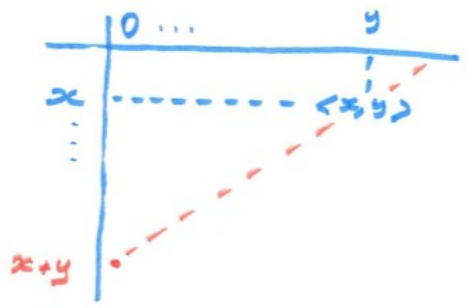
\includegraphics[scale=0.5]{images/coord_dim.png}
    \caption{Diagonale che passa per $\langle x,y\rangle $}
\end{figure}
Notiamo che per il valore che voglio valutare attraverso la funzione di Cantor passa una diagonale,
questa diagonale parte dalla colonna $0$ e dalla riga $x+y$ (il punto $\langle x+y,0\rangle $). La funzione
coppia nell'origine della diagonale assumerà un certo valore, e visto che i numeri sulla
diagonali incrementano in maniera crescente di una sola unità, allora potrò raggiungere $\langle x,y\rangle $
sommando $y$.\\A questo punto il mio problema si riduce a trovare delle coppie particolari ovvero,
la cui seconda coordinata è $0$, le chiamiamo $\langle z,0\rangle$. Notiamo nella prima colonna
c'è una correlazione con gli elementi di $x$, e vediamo che l'elemento $i$-esimo della prima
colonna corrisponde alla somma tra il corrispettivo elemento $x$ e l'elemento $i-1$ della colonna,
allora riusciamo ad esprimere una \textbf{legge matematica} per descrivere questa \textit{codifica}.

\begin{enumerate}
    \item $\langle x,y\rangle =\langle x+y,0\rangle +y$
    \item $\langle z,0\rangle ? \implies \langle z,0\rangle = \sum_{i=1}^z i+1=\frac{z(z+1)}{2}+1$
\end{enumerate}
\noindent Allora $(1)+(2)$:
$$\langle x,y\rangle = \langle x+y,0\rangle+y=\frac{(x+y)(x+y+1)}{2}+y+1$$

\paragraph{Come tornare da $\mathbb{N}^2$ a $\mathbb{N}^+$}
Ovvero, come trovare le funzioni $sin$ e $des$.
$$\langle x,y \rangle = n \longrightarrow sin(n)=x \text{ e } des(n)=y$$
\begin{figure}
    \centering
    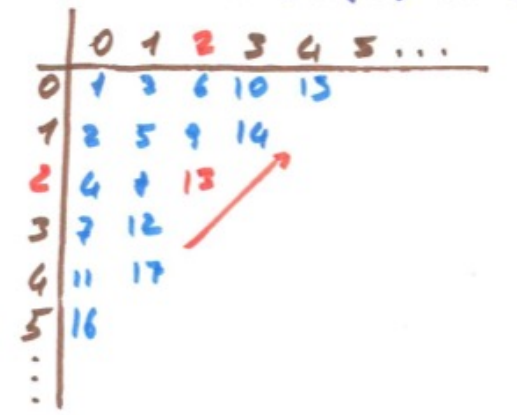
\includegraphics[scale=0.5]{images/coord_dim_2.png}
    \caption{$n=13$}
\end{figure}

Partiamo da un elemento $n$ presente nell'intersezione dei due insiemi definiti da
$x$ e $y$ e vogliamo individuare le due relative componenti. Procedo trovando
le coordinate dell'origine della diagonale che passa per $n$, ovvero $\langle\gamma ,0\rangle$.
Considerando la dimostrazione precedente possiamo dire che $y = n-\langle\gamma ,0\rangle$, ovvero
procedo a ritroso sulla diagonale partendo da $n$ ed andando verso $\langle\gamma ,0\rangle$.\\Allora,
sapendo che $\gamma=x+y$ posso trovare facilmente le parti destre e sinistre.\\ Il problema principale
ora è trovare $\gamma$, questo non è altro che l'intero più grande valore tale per cui l'origine
della diagonale sia minore di $n$.
$$\gamma = \max\{z\in\mathbb{N}:\langle z,0\rangle\leq n\}$$
Quindi dobbiamo risolvere la disuguaglianza la quale ci darà un range su $n$, all'interno di questo
range $\langle z,0\rangle\leq n$ andiamo a prendere l'intero più grande che soddisfa questa disuguaglianza.
$$\langle z,0\rangle\leq n\longrightarrow\frac{z(z+1)}{2}+1\leq n\longrightarrow z^2+z+2-2n\leq 0$$
$$z_{1,2}=\frac{-1 \pm\sqrt{8n-7}}{2}$$
Quindi devo scoprire quale è l'intero più grande dati:
$$\frac{-1 -\sqrt{8n-7}}{2}\leq z\leq \frac{-1 +\sqrt{8n-7}}{2} $$
l'elemento a destra è il più grande valore, ma non so se è intero, quindi dovrò correggere ciò:
$$\gamma=\left\lfloor\frac{-1+\sqrt{8n-7}}{z} \right\rfloor$$
Questa è un formula che utilizza la variabile in input $n$, quindi riusciamo a ricavare il parametro
sinistro e destro della funzione di Cantor e ritornare allo stato iniziale:
$$des(n)=y=n-\langle\gamma ,0\rangle \text{ e }sin(n)=x=\gamma -y$$

\paragraph{Esempio andata e ritorno tra $\mathbb{N}^2$ e $\mathbb{N}^+$}
$$\text{Andata : }\mathbb{N}^2 \longrightarrow\mathbb{N}^+$$

$$\langle 10,20\rangle = \frac{30\cdot31}{2}+20+1=15\cdot31+21=485+21=486$$

$$\text{Ritorno : }\mathbb{N}^+\longrightarrow\mathbb{N}^2$$
$$\gamma = \left\lfloor \frac{-1 + \sqrt{8 \cdot 436-7}}{2} \right\rfloor = \lfloor 30.6448\rfloor = 30$$
$$y=486- \langle 30,0\rangle = 486- \left(\frac{30\cdot31}{2}+1\right)=486-466=20=des(486)$$
$$x=30-20=10=sin(486)$$
Adesso noi abbiamo dimostrato che $\mathbb{N}^2\sim\mathbb{N}^+$.

\paragraph{Dimostrazione $\mathbb{N}\times\mathbb{N}\sim\mathbb{N}$}
Definisco una nuova funzione:
$$[,]:\mathbb{N}\times\mathbb{N}\text{ tale che }[x,y]=\langle x,y\rangle-1$$
Adesso ho una funzione esplicita per mappare $\mathbb{N}^2$ su $\mathbb{N}$.\\Nota: A questo
punto otteniamo che l'insieme dei razionali $\mathbb{Q}$ sono coppie di interi $(num,den)$. Dunque
$[,]$ mostra che $\mathbb{Q}$ è numerabile.

\paragraph{Dimostrazione rigorosa che $DATI\approxeq\mathbb{N}$}
Mostriamo le nozioni appena apprese sulle principali strutture dati.
\paragraph{Liste d'interi}\mbox{}\\
$$\textit{codifichiamo } x_1,x_2,...,x_n\rightarrow\langle x_1,x_2,...,x_n\rangle$$
Quindi il numero che rappresenta la codifica è indicato con il numero all'interno delle parentesi angolari.
L'idea consiste nell'incapsulare il risultato di una coppia di elementi come elemento destro
della coppia più esterna. Non sapendo quanto sia lunga la lista dovrò porre un elemento che mi
segnali il termine, e questo lo posso fare con $\langle x_n,0 \rangle$.

$$\langle x_1,x_2,...,x_n\rangle = \langle x_1,\langle x_2,\langle ...\langle x_n,0\rangle ...\rangle\rangle\rangle$$

\noindent Per esempio:
$$\textit{codifica }1,2,5\rightarrow\langle 1,2,5\rangle=\langle 1,\langle 2,\langle 5,0\rangle\rangle\rangle=$$
$$\langle 1,\langle2,16\rangle\rangle=\langle 1,188\rangle=$$
$$=18144$$
Per l'operazione di decodifica quello che facciamo è di considerare la codifica della mia lista $M$ (mon il
risultato ma la lista di coppie incapsulate) come un albero binario. Allora dato questo albero il figlio
sinistro è l'elemento sinistro (la testa della lista) ed il figlio destro è la parte restante della lista,
allora continuando a considerare il figlio sinistro come una struttura dati lineare ottengo
la lista codificata, questo attraversamento dell'albero in pre-ordine terminerà quando incontrerà un
figlio destro $0$ (l'ultimo elemento, c'è solo un elemento  con $0$).\\Vogliamo effettuare
delle implementazione in pseudo-codice (simile C), assumiamo $0$ come la lista nulla, e $\langle,\rangle,sin,des$
come la funzione di Cantor $\langle , \rangle$.
\paragraph{Implementazione codifica}\mbox{}
\begin{lstlisting}[mathescape=true]
int encode($x_1,...,x_n$){
    int $k$ = 0;
    for(int $i$ = $n$; $i$ >= 1; $i$--)
        $k$ = $\langle x_i,k\rangle$;
    return $k$;
}
\end{lstlisting}
\paragraph{Implementazione decodifica}\mbox{}
\begin{lstlisting}[mathescape=true]
void decode(int $n$){
    if($n$!=0){
        print($sin(n)$);
        decode($des(n)$);
    }
}
\end{lstlisting}

Altre operazioni utili possono essere sono quelle per calcolare la \textbf{lunghezza}:
\begin{lstlisting}[mathescape]
int length(int n){
    return $n$==$0$ ? $0$ : $1$ + length($des(n)$);
}
\end{lstlisting}
Oppure per calcolare la \textbf{proiezione}:
\[
    proj(t,b)=
    \begin{cases}
        -1  & \text{se } t>length(n)\text{ o }t==0                                           \\
        x_t & \text{se }1\leq t\leq length(n)\text{ e }n=\langle x_1,...,x_t,..., x_m\rangle
    \end{cases}
\]
\begin{lstlisting}[mathescape]
int proj(int $t$, int $n$){
    if ($t$ == $0$ || $t$ > length($n$))
        return $-1$;
    else {
        if ($t$ == $1$)
            return $sin(n)$;
        else
            return proj($t-1$,$des(n)$);
    }
}
\end{lstlisting}
\paragraph{Esercizi - $incr,decr$ (da implementare)}\mbox{}
\[incr(t,n)=
    \begin{cases}
        -1                                    & \text{se }t>length(n)\text{ o }t==0                                            \\
        \langle x_1, ...,x_t+1,...,x_n\rangle & \text{se } 1\leq t\leq length(n)\text{ e }n=\langle x_1,...,x_t,...,x_n\rangle
    \end{cases}
\]
$decr(t,n)=\text{ come sopra ma con }\langle x_1,...,x_t-1,...,x_m$

\paragraph{Corrispondente numerico : $DATI\sim\mathbb{N}$}\mbox{}\\
Adesso sappiamo codificare liste di interi, questo ci da un idea del fatto che i dati siano
isomorfi ad $\mathbb{N}$. Questo ci da un modo per nascondere testi, suoni, immagini dietro ad
un numero. Per esempio, per compattare un testo in un numero posso imporre una codifica (tipo
ASCII), in questa maniera posso associare un numero per ogni carattere numerico, un insieme
di caratteri numerici è codificabile utilizzando $\langle , \rangle$ il quale mi darà un
singolo numero.
\begin{figure}[H]
    \centering
    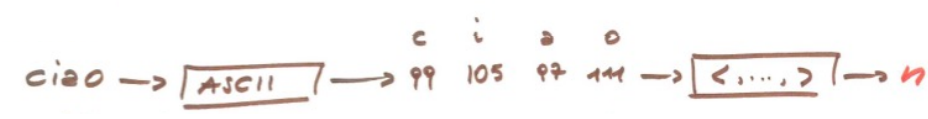
\includegraphics[scale=0.4]{images/test_codifica.png}
    \caption{Codifica di un testo}
\end{figure}
\textit{Posso usare questo modo per comprimere i testi?} In realtà questa tecnica non
è un buon compressore, questo perché la crescita del numero è quadratica rispetto
al numero di caratteri codificati (otteniamo un $n$ troppo grande e si verifica un espansione,
altroché). \textit{Perché non è un buon modo per crittografare i dati?} Il primo problema
è che il testo crittografato sarebbe molto lungo (aumenta il rischio nella perdita
di dati durante la trasmissione), secondo problema la coppia di Cantor è una funzione biettiva,
esiste un modo abbastanza diretto per tornare indietro.
\begin{figure}[H]
    \centering
    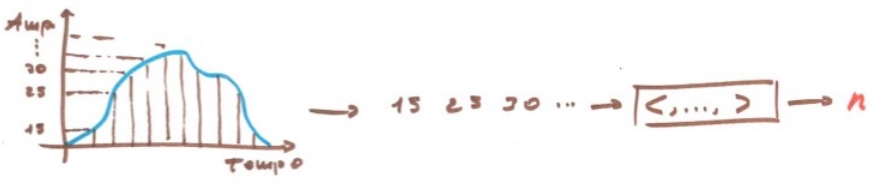
\includegraphics[scale=0.4]{images/suono_codifica.png}
    \caption{Discretizzazione del suono in segnale digitale e poi codifica in numero naturale}
\end{figure}
Per i suoni il discorso è molto simile, grazie alla \textbf{campionatura} (o
\textbf{discretizzazione}) dei segnali analogici in un segnale digitale, ovvero una grandezza
discreta sotto forma di numeri naturali.\\Per le immagini potrei usare la tecnica bitmap,
quindi per ogni bit registro un colore che verrà codificato con un numero (e da qui come per
gli altri casi sappiamo come muoverci).

\paragraph{Codifica di altre stutture dati}\mbox{}\\
Codifica di un \textbf{array} a dimensione finita, proprio per questo non necessità di
un elemento che mi ponga fine alla sequenza (so già dove fermarmi).
$$x_1,...,x_n\rightarrow[x_1,...,x_n]$$
$$[x_1,...,x_n]=[x_1,...,[x_{n-1},x_n]]...]$$
Codifica di una \textbf{matrice}, esse sono array bidimensionali dove hanno anch'esse
dimensione fissa e nota. Quindi mi basta codificare per riga le matrici e poi codificare
le codifiche.
\[
    \begin{bmatrix}
        x_{11} & x_{12} \\
        x_{21} & x_{22} \\
    \end{bmatrix}
    =\left[[x_{11},x_{12}],[x_{21},x_{22}]\right]
\]
Sia per la codifica di array che per quello delle matrici sono facilmente implementabili
le primitive numeriche ad esempio $elem(i,j,n)$ che restituisce l'elemento $(i,j)$-esimo
di una matrice codificata dal numero $n$.\\Codifica dei \textbf{grafi}, sappiamo
che un grafo è rappresentabile con lista di adiacenza, matrice di adiacenza,...
quindi possiamo codificare la lista o la matrice.
\paragraph{Conclusione}\mbox{}\\
Abbiamo mostrato effettivamente che grazie alla
corrispondenza effettiva di $DATI\sim\mathbb{N}$ che i dati possono essere "scartati" e tenuti solamente i
numeri, questo perché ogni dato può essere rappresentato con un numero naturale, questo
grazie a delle leggi matematica effettive ed implementabili, che mi
permettono di codificare e decodificare il dato.\\Quindi la nostra funzione $f:DATI\rightarrow DATI_{\bot}$
che rappresenta un qualsiasi problema può essere sostituita da una funzione $f:\mathbb{N}\rightarrow\mathbb{N}_\bot$,
ed è questo quello che i nostri calcolatori calcoleranno, quindi possiamo dire che il nostro universo
dei problemi $DATI^{DATI}_\bot$ non è altro che $\mathbb{N}^{\mathbb{N}}_\bot$

\subsubsection{Prefazione alla dimostrazione $PROG\sim\mathbb{N}$}
Per spiegare ciò utilizzeremo un linguaggio apposito detto
\textit{"linguaggio RAM"} e su un sistema formale apposito detto \textit{"sistema RAM"}.
Grazie alla semplicità di questo potrò mostrare molto semplicemente:
\begin{itemize}
    \item Che i programmi sono numerabili $PROG\sim\mathbb{N}$
    \item In maniera rigorosa la semantica dei programmi, $\mathcal{C}(P,\_)\rightarrow RAM(P,\_)$
    \item Ed altrettanto formalmente potrò definire la potenza computazionale $F(RAM)$, questo fornirà
          un idea di \textit{che cosa è calcolabile}.
\end{itemize}
Il linguaggio RAM è un \textit{assembly} molto semplificato, per questo motivo l'idea di
calcolabilità è altamente criticabile, poiché il modello potrebbe fare scappare qualcosa
per via della banalità.

Si introduce un altro modello molto più sofisticato la macchina \textit{while(JVM)}, quello
che è calcolabile è effettivamente calcolabile da questo.

Metteremo poi a confronto il modello formale $F(RAM)$ con quello sofisticato $F(while)$. Se
quest due idee di calcolabilità risultassero diverse allora la cosa è un po'
pericolosa, perchè l'dea di calcolabilità dipenderebbe dal periodo storico.
Se invece due idee così diametralmente opposte risultassero uguali, ovvero che calcolano
lo stesso insieme di funzioni, allora incomincio a capire che l'idea di calcolabilità è intrinseca
ai problemi. Ed è questo che ci porterà alla \textbf{tesi di Church} (spoiler).

Prima di arrivare a ciò dobbiamo dimostrare che $PROG\sim\mathbb{N}$, e per fare questo dobbiamo
introdurre la macchina RAM.

\subsubsection{Sistema di calcolo RAM}
L'hardware della macchina RAM:
\begin{itemize}
    \item Una \textbf{memoria} $R$ costituita contigua di registri, ognuno di questi registri può memorizzare
          i numeri naturali arbitrariamente grandi (non hanno una capienza).
          Il registro $R1$ è il registro di input; $R0$ registro di output.

    \item Il \textbf{program counter} $L$, un registro contenente l'indirizzo dell prossima
          istruzione da eseguire.

    \item Un \textbf{programma} $P$, costituito da una  sequenza di istruzioni, un istruzione RAM può essere:
          \begin{itemize}
              \item Incremento: $R_k \leftarrow R_k +1$
              \item Decremento: $R_k \leftarrow R_k -1$ (non può mai andare sotto lo zero)
                    \[
                        x-y=
                        \begin{cases}
                            x-y & \text{se } x\geq y \\
                            0   & \text{altrimenti}
                        \end{cases}
                    \]
              \item Salto condizionato: $\text{IF } R_k=0\text{ THEN GOTO } m, m\in{1,...,|P|}$
          \end{itemize}
\end{itemize}
\paragraph{Esecuzione su una macchina RAM}
\begin{enumerate}
    \item Fase di inizializzazione del programma $P$.
    \item Si carica il dato $m$ nel registro di output $R_1$.
    \item Si comincia ad eseguire l'istruzione al posto $1$, e man mano
          il PC continua ad incrementare così da poi eseguire l'istruzione successiva
          (eccetto nel caso in cui non si incontri un istruzione di salto).
    \item Per convenzione la macchina si arresta quanto ik PC il numero $0$
          $$L=0\implies HALT$$
          c'è possibilità per via dell'istruzione di salto di mandare in loop
          l'esecuzione della macchina.
    \item L'output di questo programma dato un input $x$ ha due possibilità
          \begin{itemize}
              \item Il programma si ferma ($HALT$) e l'output è presente all'interno del registro $R_0$.
              \item Il programma non termina, allora in questo caso l'output
                    per l'input sarà indefinito
          \end{itemize}
          Quello che fa il programma è calcolare una funzione:
          $$\varphi(x)=cout(R_0)/\bot$$
          Chiameremo \textbf{semantica del programma $P$}:
          $$\varphi_p = \mathbb{N}\rightarrow\mathbb{N}_\bot$$
\end{enumerate}
Questa è una definizione di semantica del programma molto intuitiva, quello che voglio
fare però è utilizzare degli oggetti matematici con i quali specificare
in maniera formale e corretta la semantica del programma.

\paragraph{Definizione formale di semantica di un programma RAM}\mbox{}\\
Introduciamo il concetto di \textbf{semantica operazionale}, questo è il tipo di semantica
più semplice. Significa specificare che cosa fa una data istruzione andando a vedere quale
è l'effetto di quell'istruzione sulla data macchina.

Per descrivere l'effetto di un istruzione, prendiamo una foto della macchina prima dell'esecuzione
e dopo. La "foto" solitamente si chiama \textbf{stato} della macchina. Quindi spiego la semantica
di una istruzione specificando il cambiamento di stato indotto dall'esecuzione di quell'istruzione.
Questo significa dare la semantica operazionale di una macchina.
\begin{figure}[H]
    \centering
    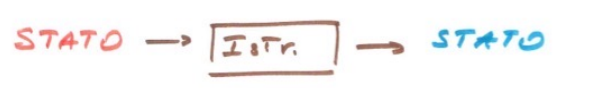
\includegraphics[scale=0.5]{images/cambio_stato.png}
\end{figure}

\paragraph{Esecuzione di un programma $P$ e sua semantica}
L'esecuzione di un programma consiste nell'esecuzione di molteplici cambiamenti di stato a partire
dallo stato iniziale $S_{init}$ (partendo un inpput $n$)
e giungendo a quello finale $S_{final}$. Si dice che la computazione
di $P$ induce una sequenza di stati.

\begin{figure}[H]
    \centering
    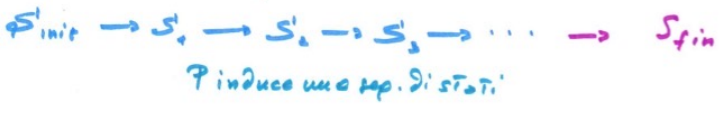
\includegraphics[scale=0.5]{images/stati_seq.png}
    \caption{Sequenza di stati indotta da $P$}
\end{figure}
\begin{figure}[H]
    \centering
    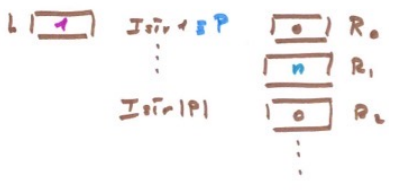
\includegraphics[scale=0.5]{images/stato_init.png}
    \caption{Situazione globale durante $S_{init}$}
\end{figure}
\begin{figure}[H]
    \centering
    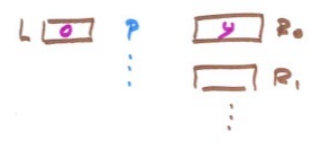
\includegraphics[scale=0.5]{images/stato_fina.png}
    \caption{Situazione globale durante $S_{final}$ (in caso di $HALT$)}
\end{figure}
Quindi la semantica del programma sarà:
\[
    \varphi_p(x) =
    \begin{cases}
        y \\
        \bot
    \end{cases}
\]
Dove $\bot$ mi indica una sequenza infinita di stati in loop.
\paragraph{Ingredienti della definizione formale della semantica}\mbox{}\\
\begin{itemize}
    \item \textbf{Stato} di una macchina RAM, è lo stato dei registri di quella macchina.
          Matematicamente modella to come una funzione che mi restituisce il contenuto
          del risultato quando la macchine è nello stato $S$
          $$S:\{L, R_i\}\implies\mathbb{N}$$
          $$STATI=\mathbb{N}^{\{L,R_i\}}=\{\text{insieme di tutti i possibili stati della macchina}\}$$
          $$S(R_j) = \textit{contenuto di } R_j\text{ durante lo stato } S$$

    \item \textbf{Stato finale} della macchina RAM, uno stato tale per cui:$$S(L)=0\implies HALT$$
    \item \textbf{Dato}, rappresentato da $\mathbb{N}$, questo perchè sappiamo che $\mathbb{N}\sim DATI$.
    \item \textbf{Inizializzazione}, dato il dato $n$ prepara la macchina nell ostato iniziale
          con input $n$. Quindi sarà una funzione $in$ questa creerà uno stato $S_{init}$ a partire
          da un input $n$:
          $$in:DATI\rightarrow STATI \text{ t.c. } in(n)=S_{init}$$
          Essa imposterà il contenuto del primo registro ad $1$, e tutti gli altri a $0$, e poi
          il caricherà nel program counter l'indirizzo della prima istruzione (contenuto
          del registro).
          \[
              S_{init}(R_i)=
              \begin{cases}
                  n & \text{se } i=1 \\
                  0 & \text{se } i=0
              \end{cases}
          \]
          $$S_{init}(L)=1$$

    \item \textbf{Programmi}, insieme dei programmi RAM $PROG=\{\text{programmi RAM}\}$, un
          singolo programma $P\in PROG$, tale per cui la sua cardinalità indica
          il numero di istruzioni contenute $|P| = \#istr$.
    \item \textbf{Esecuzione}, essa mi specifica la dinamica del programma che mi fa
          passare da uno stato al successivo. Questo è possibile con utilizzando la \textit{funzione
              stato prossimo} $\delta$. Tale funzione mi permette di spostarmi dallo stato attuale
          $S$ a quello successivo $S'$.
          $$\delta:STATI\times PROG \rightarrow STATI_\bot$$
          $$\delta(S,P)=S'$$
          Lo stato prossimo dipenderà dall'istruzione che in quel momento deve essere eseguita,
          e per conoscere tale istruzione devo andare a vedere il contenuto del program counter
          allo stato attuale $S(L)$ (quindi lo stato prossimo dipenderà da $S(L)$).\\\textit{Come
              è definito lo stato prossimo in funzione dello stato attuale?}
          \begin{enumerate}
              \item Se $S(L)=0$ (ovvero in terminazione), allora lo stato prossimo non è definito
                    $S'=\bot$.
              \item Se $S(L)>|P|$, significa che abbiamo superato l'ultima istruzione
                    e che il program counter è stato incrementato diventando così più
                    grande del numero di istruzioni del programma. Quello che si fa è:
                    $$S'(L)=0\text{ HALT}$$
                    $$\forall i:S'(R_i)=S(R_i)$$
              \item Se $1\leq S(L)\leq |P|$, questo è il caso comune e considerando
                    la $S(L)$-esima istruzione:
                    \begin{itemize}
                        \item $R_k\leftarrow R_k \pm 1$, definite come:
                              \begin{lstlisting}[mathescape=true]
$S'(R_k) = S(R_k) \pm 1$
$S'(L)=S(L)+1$
$S'(R_i)=S(R_i)\text{ con } i\neq k$
                        \end{lstlisting}
                        \item $\text{IF }R_k=0\text{ THEN GOTO }m$, definita come:
                              \begin{lstlisting}[mathescape]
$S'(R_i) = S(R_i)$
if $S(R_k)==0$ then
    $S'(L)=m$
else
    $S'(L)=S(L)+1$
                        \end{lstlisting}
                    \end{itemize}
          \end{enumerate}
          \paragraph{Esecuzione del programma $P\in PROG$}\mbox{}\\
          Ora posso definire la sequenza di computazione di un programma $P\in PROG$ su un input $n\in\mathbb{N}$.
          Una computazione è una sequenza di stati indotta dalla dinamica:
          $$in(n)=S_0, S_1,...,S_i,S_{i+1},...$$
          Eventualmente la sequenza può essere infinita (loop), o terminare se un $S_m$
          raggiunge un $S_m(L)=0$ (halt).

          Dobbiamo vincolare la sequenza di stati alla funzione $\delta (S,P)$,
          e dire che per ogni $\delta(S_i,P)= S_{i+1}$.

          Quindi, la semantica di $P$, è definita come $\varphi_P:\mathbb{N}\rightarrow\mathbb{N}_\bot$:
          \[
              \varphi_P(n)=
              \begin{cases}
                  y    & \parbox[t]{.6\textwidth}{se la computazione del programma termina in con  S(L)=0
                  ed il contenuto di $S_m(R_0)=y$}                                                        \\
                  \bot & \text{ se la computazione del programma va in loop}
              \end{cases}
          \]
\end{itemize}
Ora posso definire formalmente la potenza computazionale del sistema RAM:
$$F(RAM)=\{f\in\mathbb{N}^{\mathbb{N}}:\exists P\in PROG,\varphi_P = f\}=\{\varphi_P : P\in PROG\}\nsubseteq\mathbb{N}^{\mathbb{N}}_{\bot}$$
Ovvero tutte le funzioni per cui esiste un programma $P$ tale per cui $\varphi_P = f$ (o $\varphi_P$ al variare di $P$).

\paragraph{Alcuni programmi RAM e le loro funzioni che vengono calcolate}\mbox{}
\begin{figure}[H]
    \centering
    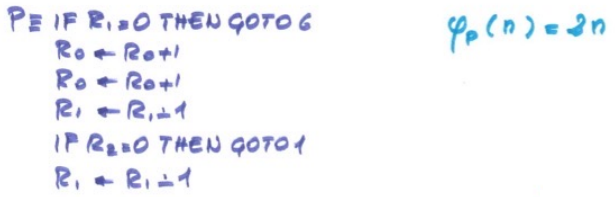
\includegraphics[scale=0.5]{images/2n.png}
    \caption{$n$}
\end{figure}

\begin{figure}[H]
    \centering
    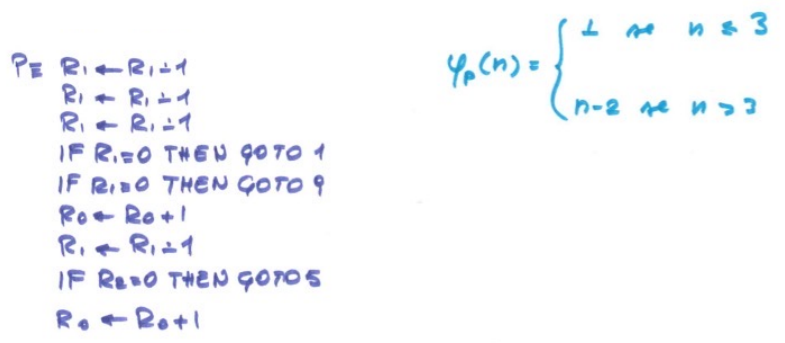
\includegraphics[scale=0.5]{images/n_complx.png}
    \caption{Funzione più complicata}
\end{figure}

Questi programmi possono essere spiegati formalmente con gli strumenti matematici precedentemente
forniti, per esempio con il primo programma:

\begin{figure}[H]
    \centering
    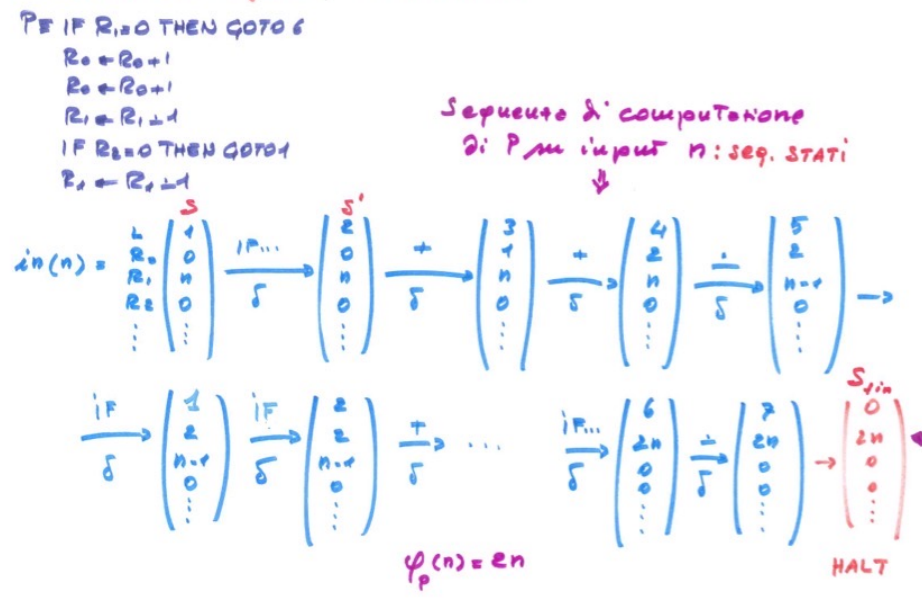
\includegraphics[scale=0.4]{images/n_formale.png}
    \caption{Rappresentazione formale di $\varphi_P(n)=2n$}
\end{figure}

Questo è il modo corretto di procedere, e questo modo permette di definire formalmente
la potenza computazionale di una macchina RAM, non lasciando nulla al caso.

\paragraph{Alcune considerazioni}
\begin{itemize}
    \item $F(RAM)$ \textit{conterrà funzioni più complesse o solo quelle banali?} In realtà
          si posso fare delle funzioni più complesse, questo comunque è un primo
          tentativo di fare qualcosa di ragionevole che mi permette la completa formalizzazione.
    \item Indubbiamente la semplicità di questo sistema di calcolo ci permette l'estrema
          formalizzazione, tale che vedremo che sarà possibile dimostrare $PROG\sim\mathbb{N}$
\end{itemize}

\subsubsection{Dimostrazione $PROG\sim\mathbb{N}$}
Dato un programma RAM vogliamo associare un numero a tale programma
in maniera che partendo quel numero sia possibile tornare al sorgente.

Ovvero vogliamo dimostrare che anche i programmi possono essere in corrispondenza biunivoca
con i numeri naturali (utilizzeremo la semplicità della macchina RAM).

$$P\equiv Istr_1,Istr_2,...,Istr_m$$
Il primo passo consiste nell'aritmetizzazione dell'istruzione, ovvero trasformare una lista
di istruzioni in una lista di codici numerici. Successivamente utilizzando la funzione lista
di Cantor possiamo trasformare questo elenco di codici in un singolo numero $n$.
\begin{figure}[H]
    \centering
    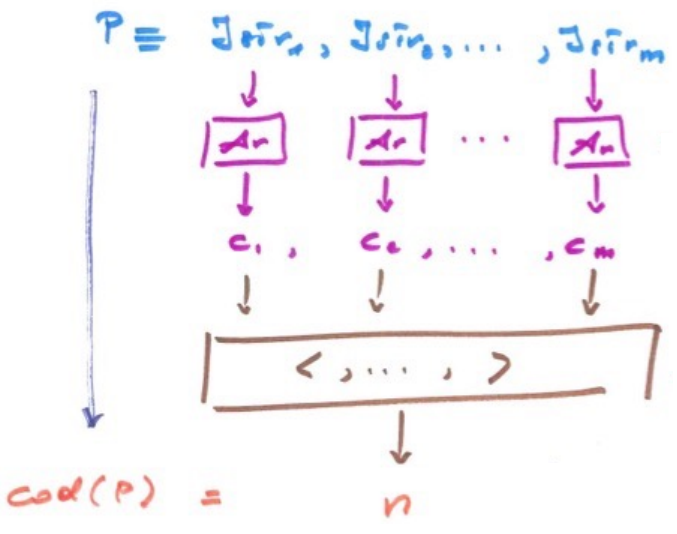
\includegraphics[scale=0.5]{images/PROG_to_num.png}
\end{figure}
Sappiamo che la funzione lista di Cantor è invertibile quindi possiamo ricostruire le codifiche
associate alle istruzioni. Ora se l'operazione di aritmetizzazione del sorgente è
invertibile, allora ci sarà possibile risalire al sorgente partendo da $n$.

In generale un procedimento che fa corrispondere ad una qualsiasi struttura matematica
un numero, si chiama operazione di \textbf{aritmetizzazione} o \textbf{Godelizzazione}.

Il nostro scopo è quello di aritmetizzare ogni istruzione.

\paragraph{Aritmetizzare biunivocamente le istruzioni RAM}
$$Ar:Istr\rightarrow\mathbb{N}\text{ e }Ar^{-1}:\mathbb{N}\rightarrow Istr\text{ t.c. }
    Ar(Istr)=n\Leftrightarrow Ar^{-1}(n)=Istr$$
Nel caso di un programma RAM significa aritmetizzare tre tipi di istruzioni.
$$Ar(R_n\leftarrow R_n+1)=3k$$
$$Ar(R_n\leftarrow R_n-1)=3k+1$$
$$Ar(\text{If }R_k=0\text{ then goto }m)=3\langle k,m\rangle-1$$

Come è fatta $Ar^{-1}$? La funzione di decodifica è biunivoca ? La funzione
risulta sia iniettiva che suriettiva, l'applicazione di questa funzione è permessa
attraverso l'operatore di modulo per $3$.
\begin{figure}[H]
    \centering
    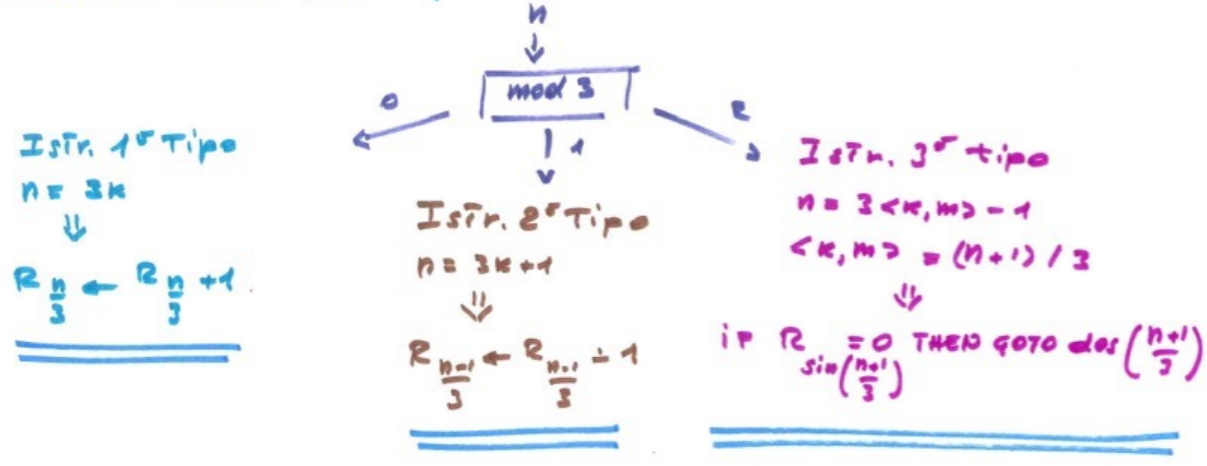
\includegraphics[scale=0.4]{images/mod3.png}
\end{figure}

Ricapitolando, il passaggio da programmi a numeri è molto semplice
$$cod(P)=\langle Ar(Istr_1),...,Ar(Istr_m)\rangle$$
mentre il passaggio da numeri a programmi, parto da $n$ e trovo la parte sinistra e
la parte destra. Vediamo passo per passo:

\begin{figure}[H]
    \centering
    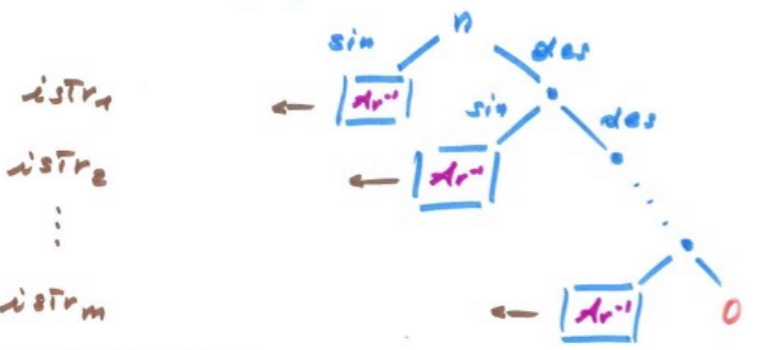
\includegraphics[scale=0.5]{images/decod_bin.png}
\end{figure}

Al primo passo dalla parte sinistra trovo il codice della prima istruzione
(aritmetizzato), quindi nel caso in cui io voglia il sorgente del programma
quello che devo fare è applicare $Ar^{-1}$ sulla parte sinistra. Questo finché
non si incontra il terminatore sul figlio destro.\\Se io volessi sempre
scompattare il programma $P$ e dato $n$ io volessi sapere il numero di istruzioni
del programma $|P|$, che cosa devo calcolare?
$$|P|=length(cod(P))$$
Abbiamo quindi dimostrato in maniera inequivocabile il secondo tassello, ovvero
che i programmi sono equinumerosi rispetto ai numeri naturali.
$$PROG\sim\mathbb{N}$$

Adesso che abbiamo acquisito gli strumenti, proviamo a vedere ad occhio qualche
esempio.

\paragraph{Primo programma RAM}\mbox{}\\
\begin{figure}[H]
    \centering
    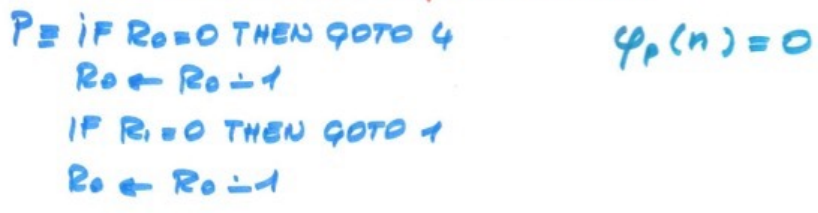
\includegraphics[scale=0.5]{images/prog_1.png}
\end{figure}

La corrispettiva aritmetizzazione delle istruzioni :

\begin{figure}[H]
    \centering
    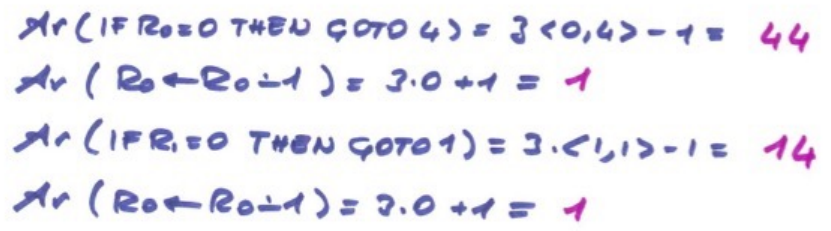
\includegraphics[scale=0.5]{images/cod_1.png}
\end{figure}
$$cod(P)=\langle 44,\langle 1,\langle 14,\langle 1,0\rangle\rangle\rangle\rangle=50556496$$
Questo non è un ottimo modo per compattare i programmi ram, poiché cresce esponenzialmente
rispetto al programma. Tuttavia questo ha scopi didattici.
$$\varphi_{50556496}(n)=0$$

\paragraph{Sorgente RAM da un numero}\mbox{}\\
Il numero è il 311, ha come parte sinistra 14 e come parte destra 10. Facendo il modulo 3
del figlio sinistro otteniamo otteniamo 2, quindi si tratta di un istruzione condizionale,
in questo caso troviamo che il valore dell coppia di Cantor $\langle k,m\rangle = 5$. Quindi
dobbiamo trovare il figlio sinistro e destri di $5$, che sono entrambi $1$. Quindi
la prima istruzione sarà:
$$\text{If }R_1=0\text{ then goto }1$$
\begin{figure}[H]
    \centering
    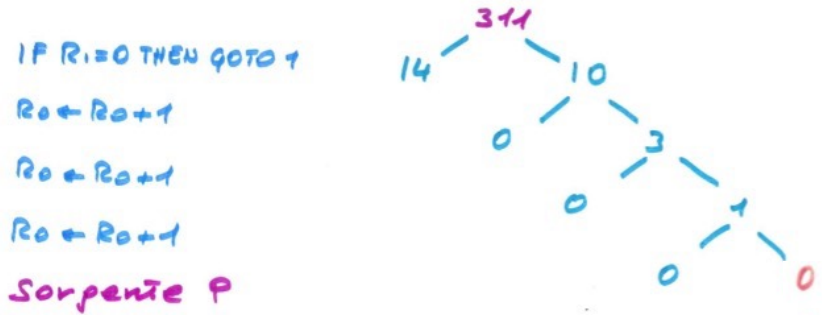
\includegraphics[scale=0.5]{images/sorgente_p.png}

\end{figure}
Quale é la semantica di questo programma ? (ovvero $\varphi_P(n)$)
\[
    \varphi_P(n)=\varphi_{311}(n)=
    \begin{cases}
        \bot & \text{se }n=0 \\
        3    & \text{se }n>0
    \end{cases}
\]
Se l'input $n$ è 0 vado in loop, poiché continuo a rieseguire la stessa istruzione,
altrimenti parto dalla terza istruzione.

\paragraph{Riflessioni su $PROG\sim\mathbb{N}$}
\begin{itemize}
    \item Abbiamo dimostrato che i numeri sono un linguaggio di programmazione, questo
          perché un numero può rappresentare un linguaggio.

    \item $F(RAM)=\{\varphi_P :P\in PROG\}$, la potenzia computazionale del sistema di programmazione
          RAM, adesso la posso scrivere come $F(RAM)=\{\varphi_i\}_{i\in\mathbb{N}}$ questo mostra ina maniera inequivocabile che la potenza
          computazionale della macchina RAM è enumerabile.

    \item Per il sistema RAM si ha rigorosamente che $F(RAM)\sim\mathbb{N}\nsim\mathbb{N}^{\mathbb{N}^\mathbb{N}}$,

    \item Questa è una prima idea di calcolabilità, esploriamo un sistema di calcolo $\mathcal{C}$ più complesso
          e vediamo la sua potenza computazionale di questo, e vediamo se è più complessa. Questo va fatto è onestamente
          dire che ciò che è calcolabile sia $F(RAM)$ è troppo restrittivo.

    \item Possiamo avere che questo sistema di clacolo più avanzato ampli l'insieme $F(RAM)$.
\end{itemize}

\subsubsection{Il sistema di calcolo While}
Il linguaggio è basato su un linguaggio moderno, contrapposto all'assembly della macchina RAM (quindi
anni 50'), adesso ci troviamo nell'utilizzo di un linguaggio strutturato.

Hardware:
\begin{itemize}
    \item \textbf{Memoria} costituita da 21 registri. Siccome parliamo di linguaggio strutturato
          non si parla più con il termine registri ma ci si riferirà con \textit{variabili}.
          $$x_0,x_1,...,x_{20}$$. La variabile $x_1$ ci si troverà l'input del programma, mentre
          l'output si troverà su $x_0$.
    \item Program counter non presente, poiché si parla di linguaggio strutturato, ed in questo
          le istruzioni vengono eseguite una dopo l'altra (punti di inizio ciclo e finale
          sono ben definiti, ed il \textit{goto} non è presente).
\end{itemize}
20 variabili potrebbero sembrare poche, in realtà la numerosità dei dati non è un problema
poiché abbiamo primitive che mi permettono di condensare (coppia di Cantor) un infinità
di variabili.\\Il linguaggio while ha una sintassi induttiva (dove i costrutti dei linguaggi
sono definiti su delle basi semplici, i mattoni, e man mano costruisco istruzioni più
complesse):
\begin{itemize}
    \item Comando di \textbf{assegnamento}: $x_k:=0 x_k:=x_j+1 x_k:=x_j-1$
    \item Comando \textbf{while}: $\text{while }x_k\neq 0\text{ do } G$, dove $G$
          ovvero il corpo del loop, può essere un comando di assegnamento, while o composto.
    \item Comando \textbf{composto}: $\underline{\text{begin }}C_1; C_2; ...;C_m;
              \underline{\text{ end}}$ dove la sequenza è composta da comandi che possono essere
          di assegnamento, while o composto.
\end{itemize}
Come si può vedere sono strutture che sono in grado di nascondere altre strutture, di per sè
un programma while è un comando composto.\\Indicheremo com $W-PROG=\{\text{programmi WHILE}\}$
come l'insieme dei programmi WHILE, dove ciascuno è un programma costruito induttivamente.

\paragraph{Esempio di programma WHILE}\mbox{}\\
\begin{figure}[H]
    \centering
    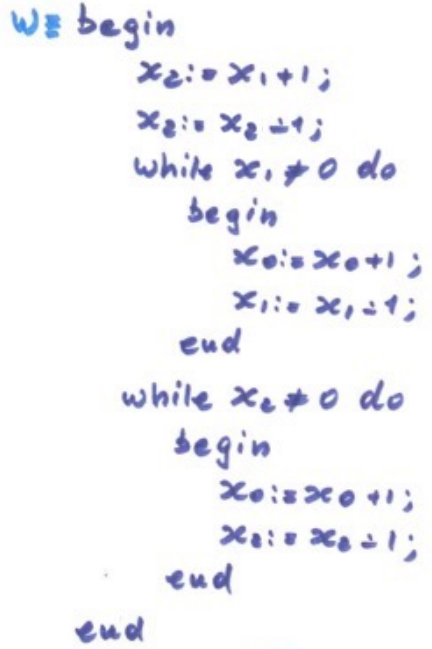
\includegraphics[scale=0.5]{images/esempio_prog_while.png}
\end{figure}
Indicheremo con $\psi_w$ le semantiche dei programmi WHILE (in questo caso il programma $w$).
$$\psi_w :\mathbb{N}\rightarrow\mathbb{N}_\bot$$
$$\psi_w (x)=2x$$

Le prime due istruzioni sono messe perché non è possibile effettuare una copia diretta,
non stiamo utilizzando il linguaggio di programmazione RAM.

Il parsing del programma ne rivela la struttura induttiva,
W-PROG è un insieme definito induttivamente (ovvero partendo
dalla base ed utilizzando dei passi induttivi): per dimostrare una proprietà $P$ su W-PROG:
\begin{enumerate}
    \item Dimostro che $P$ vale sui comandi base (passo base).

    \item Suppongo vero quella proprietà $P$ sui comandi $C$ base, e
          poi dimostro che vale sul comando più complesso $\text{while }x_n\neq 0\text{ do } C$
          (passo induttivo).

    \item Suppongo vera $P$ su $C_1,...,C_m$ e la dimostro vera su $\underline{\text{begin}}\text{ }
              C_1;...;C_m\text{ }\underline{\text{end}}$
\end{enumerate}

Quando abbiamo di fronte una struttura induttiva il modo migliore per dimostrare che una certa proprietà valaga su tutti
gli elementi della struttura dobbiamo farlo per induzione (in questo caso si parla di \textbf{induzione strutturale}).

\paragraph{Esempio}\mbox{}\\
L'insieme degli alberi binari è un insieme definito induttivamente. Sappiamo che è un DAG.
\begin{figure}[H]
    \centering
    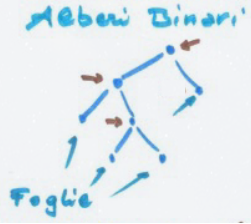
\includegraphics[scale=0.5]{images/BT.png}
    \label{fig:bt}
\end{figure}
Possiamo definire l'insieme degli alberi binari come l'insieme di tutti gli oggetti composti come
mostrato in figura \ref{fig:bt}. Oppure, possiamo definirli induttivamente

\begin{itemize}
    \item Base: Un nodo solo è considerabile un albero binario (con una singola foglia).
    \item Induzione: Se $T_1$ e $T_2$ sono alberi binari anche
          \begin{figure}[H]
              \centering
              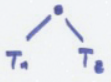
\includegraphics[scale=0.6]{images/BT_1.png}
              \caption{Binary Tree (indicati i nodi interni con le frecce marroni)}
          \end{figure}
    \item Nient'altro è un albero binario.
\end{itemize}
Allora vogliamo dimostrare pre induzione la proprietà $P$, tale che:
$$P\equiv \parbox[t]{.6\textwidth}{"Su ogni albero binario, il numero dei nodi interni è minore di uno rispetto
        a quello delle foglie."}$$

Allora dimostriamola per induzione:
\begin{itemize}
    \item Base: \textit{è vero che se ho un solo nodo la proprietà $P$ è vera?} Si poiché
          nodi interni non sono presenti.
    \item Induzione: supponiamo vera $P$ su $T_1,T_2$
          \begin{itemize}
              \item $T_1$: foglie $f_1$ foglie e $f_1-1$ nodi interni.
              \item $T_2$: foglie $f_2$ foglie e $f_2-1$ nodi interni.
          \end{itemize}

          Per esempio, prendiamo questo albero:
          \begin{figure}[H]
              \centering
              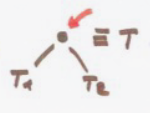
\includegraphics[scale=0.6]{images/BT_2.png}
          \end{figure}
          notiamo che il numero di foglie è pari a $f_1+f_2$. Adesso la domanda fondamentale è la seguente
          \textit{quanti nodi interni ha questo albero?} Il numero di nodi interni è pari alla somma tra i nodi
          interni di $T_1$ con quelli di $T_2$. Ma questo riutilizzando i mattoncini basilari non è altro che
          $$(f_1-1) + (f_2-1) + 1 = f_1 + f_2 -1$$
          $P$ risulta dimostrata per induzione su tutta la struttura.
\end{itemize}

\paragraph{Esempio 2}\mbox{}\\
Voglio definire una funzione $depth: \tau\rightarrow\mathbb{N}$ su un albero binario che
dato un qualsiasi albero binario mi restituisce la \textbf{profondità}: ovvero, la lunghezza del
cammino più lungo dalla radice ad una foglia dell'albero.
\begin{figure}[H]
    \centering
    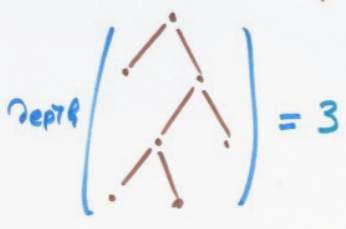
\includegraphics[scale=0.6]{images/profondità.png}
    \caption{Definizione grafica}
\end{figure}
Questa è una possibile definizione, oppure potremmo definirla induttivamente:
\begin{enumerate}
    \item Base: Dato un BT costituito da una sola radice darà $depth=0$
    \item Induzione: Dato questo albero binario
          \begin{figure}[H]
              \centering
              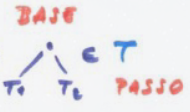
\includegraphics[scale=0.6]{images/passo_ind_depth.png}
          \end{figure}
          si prende la profondità maggiore due due sotto alberi più uno, ovvero il nuovo livello
          $depth=1+max\{depth(T_1),depth(T_2)\}$
    \item Nient'altro è in $\tau$
\end{enumerate}

\paragraph{Esecuzione su una macchina WHILE}\mbox{}\\
Considerando un input $n$
\begin{itemize}
    \item La prima è una fase di inizializzazione, quindi si avvia la macchina con il nostro
          programma $w$, dove tutte i registri della variabili sono inizializzati a 0, tranne per il registro
          in input $x_1$ che contiene $n$.

    \item Si comincia ad eseguire il programma $w$, sequenzialmente sulle istruzioni, in questo caso non
          c'è assolutamente bisogno di program counter (motivi già spiegati).

    \item Possiamo avere due casi, o l'esecuzione effettivamente termina o si incappa in un loop (while true).
          Nel primo caso l'output lo andiamo a leggere nella variabile $x_0$ (se HALT), altrimenti diciamo che è indefinito
          $\bot$. Definendo così la semantica del programma $w$, $\psi_w(n)=cont(x_0)/\bot$.
\end{itemize}

Vogliamo essere precisi anche in questo caso, ed espandere il discorso della sequenza di istruzioni durante l'esecuzione
di un programma WHILE (introducendo anche qui il concetto di stato).

\subsubsection{Definizione formale di semantica di un programma WHILE}
\begin{itemize}
    \item \textbf{Stato}, una foto dove compare in maniera completa tutto ciò che accade sulla macchina in quel dato istante.
          Rispetto alla macchina RAM lo stato viene definito in maniera differente, dal punto di vista matematico uno stato è
          una tupla di 21 elementi $(c_0, ..., c_{20})$. Detto ciò, l'insieme di tutti i possibili stati $w-stati$ è composto
          da $\mathbb{N}^{21}$ ovvero tutte le possibili 21-tuple (tuple di lunghezza 21) infinite.

    \item \textbf{Dati}, sono l'insieme dei numeri naturali.
    \item \textbf{Inizializzazione}, sta volta la funzione può essere modellata su 21 elementi, la funzione prende un
          numero e restituisce uno stato
          $$w-in:\mathbb{N}\rightarrow\mathbb{N}^{21}\text{ con }w-in(n)=(0,n,0,...,0)$$
    \item \textbf{Semantica operazionale}
          $$[]():w-com\times w-stati\rightarrow w-stati_\bot$$
          Dato un comando while $C$ e uno stato $\underline{x}$, allora
          $$[c](\underline{x})=\underline{y}$$
          sarà la funzione stato prossimo dove $\underline{y}$ è lo stato prossimo di $\underline{x}$ a seguito
          dall'esecuzione del comando $C$.
          Ovviamente possiamo definire induttivamente $[C](\underline{x})$ sulla struttura induttiva
          del comando $C$.
\end{itemize}

\subsubsection{Definizione induttiva della semantica while}
\begin{itemize}
    \item Base: gli \textbf{assegnamenti}
          \[
              [x_k=0](\underline{x})=\underline{y}\text{ con }y_i=
              \begin{cases}
                  x_i & \text{se }i\neq k \\
                  0   & \text{se }i=k
              \end{cases}
          \]

          \[
              [x_k:=x:j \pm 1](\underline{x})=\underline{y}\text{ con }y_i=
              \begin{cases}
                  x_i       & \text{se } i\neq k \\
                  x_j \pm 1 & \text{se } i=k
              \end{cases}
          \]


    \item Passo:
          \begin{itemize}
              \item Comando \textbf{composto}
                    $$[\underline{\text{begin}}\;C_1;...;C_m;\underline{\text{end}}](\underline{x})$$
                    induttivamente conosco la semantica di ciascuno di questi programmi, come essi agiscono.
                    Allora posso definire la semantica di questo comando come:

                    $$[C_m](\dots([C_2]([C_1](\underline{x})))\dots)=\underline{y}=[C_1]$$
                    Quindi l'applicazione del primo comando (che provoca cambiamento di stato)
                    sullo stato iniziale, seguita iterativamente dall'applicazione degli $m$ comandi
                    sugli stati risultanti.

              \item Comando \textbf{while}
                    $$[\text{while }x_k\neq 0 \text{ do }C](\underline{x})$$, anche qui conosco
                    per ipotesi induttiva la semantica del comando $C$.

                    $$[C](\dots([C]([C](\underline{x})))\dots)=\underline{y}=[C_1]\text{ e }...\text{ e }[C_m](\underline{x})$$
                    Il numero di volte che applicherò il comando $C$ quante volte serve per azzerare il contenuto di $x_k$
                    \[
                        =\begin{cases}
                            [C]^e(\underline{x}) & \text{con }\mu t \text{ k-esima componente di }[C]^{(t)}(\underline{k})=0 \\
                            \bot                 & \text{altrimenti}
                        \end{cases}
                    \]
                    Ovvero il più piccolo numero di volte che mi serve per azzerare la componente $k$-esima, altrimenti
                    vado in un loop interminabile.
          \end{itemize}

    \item Semantica di $W$ e $W-PROG$: a questo punto so definire in maniera formale la semantica
          di un programma while, prendiamo il programma while $w$ (il quale è un comando composto).

          Quindi è la semantica del comando composto che rappresenta $w$, quindi non è altro che preparare
          la macchina su input $x$.

          $$\Psi_w(x)=Pro(0,[w](w-in(x)))$$
          Ovvero la proiezione 0-esima dell'esecuzione del comando composto di $w$ dato uno stato finale $x$ (avviato
          da uno stato iniziale),
          significa che se il programma termina devo pescare il contenuto di $x_0$ (la proiezione di uno stato finale
          di un programma $w$).
          Nel caso in cui non avvenisse l'HALT allora avrò una semantica indefinita $\bot$.
\end{itemize}

\paragraph{Esempio di semantica di un piccolo programma while}\mbox{}\\
\begin{figure}[H]
    \centering
    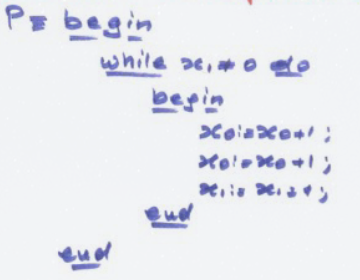
\includegraphics[scale=0.7]{images/smallprog.png}
    \caption{Programma che calcola $2n$}
\end{figure}

\begin{figure}[H]
    \centering
    \includegraphics[scale=0.7]{images/comanodwhiòe.png}
    \caption{Deduzione della semantica $\Psi_w$}
\end{figure}

\paragraph{Potenza computazionale del sistema while}\mbox{}\\
$$F(WHILE)=\{f\in\mathbb{N}_\bot^\mathbb{N} : \exists w\in w-PROG, f=\Psi_w\}=\{\Psi_w : w\in w-PROG\}$$
Definiamo la potenza computazionale di
una macchina while come l'insieme di tutte le funzioni per cui
esiste un programma while per cui si può calcolare quella funzione.Naturalmente la domanda è: \textit{che relazione esiste tra $F(RAM)$ e -$F(WHILE)$?}, quindi
che cosa è calcolabile di questi due sistemi? $\{\varphi_P:P\in PROG\}$?
Magari la macchina WHILE mi fornisce più potenza della macchina RAM? L'unico modo di scoprirlo
è confrontando le due idee. Quali situazioni si possono verificare:
\begin{enumerate}
    \item Una situazione dove $F(RAM)\nsubseteq F(WHILE)$ (inclusione propria) ovvero, che ci sono funzioni
          calcolabili con i programmi WHILE che non sono calcolabili sulle macchine RAM.

    \item Le due idee di calcolabilità non sono confrontabili, ovvero un intersezione tra i due insiemi
          dove magari alcune funzioni sono calcolabili da entrambe le architetture, oppure sono due insiemi
          totalmente disgiunti. In entrambi i casi siamo preoccupati, perché l'idea di calcolabilità è dipendente
          dal modello di calcolo adottato.

    \item Una situazione dove $F(WHILE)\nsubseteq F(RAM)$ questo sarebbe sorprendente, la macchina
          sofisticata non riesce a calcolare delle funzioni più semplici.

    \item Una situazione dove $F(WHILE)=F(RAM)$, ovvero due cose filosoficamente diverse eppure entrambe
          riescono a calcolare la stessa classe di funzioni, questo sarebbe molto interessante, perché allora
          vuol dire che calcolabile non dipende dalla tecnologia-
\end{enumerate}
Adesso dobbiamo cercare di capire quali tra i seguenti punti è quello veritiero.

\paragraph{Confrontiamo $F(RAM)$ e $F(WHILE)$}\mbox{}\\
Iniziamo con il confrontare $F(RAM)$ e $F(WHILE)$ introducendo due sistemi di calcolo $\mathcal{C}_1$ e $\mathcal{C}_2$
con i loro relativi linguaggi di programmazione. Attraverso i quali riusciamo a scrivere l'insieme dei
programmi scritti con i relativi linguaggi $\mathcal{C}_1-PROG$ e $\mathcal{C}_2-PROG$. Le relative
potenze computazioneli

$$F(\mathcal{C}_1)=\{f\in\mathbb{N}_\bot^\mathbb{N}: f=\Psi_{P_1}\text{ per qualche }P_1\in\mathcal{C}_1-PROG\}=\{\Psi_{P_1}:P_1\in\mathcal{C}_1-PROG\}$$
$$F(\mathcal{C}_2)=\{f\in\mathbb{N}_\bot^\mathbb{N}: f=\Psi_{P_2}\text{ per qualche }P_2\in\mathcal{C}_2-PROG\}=\{\Psi_{P_2}:P_2\in\mathcal{C}_2-PROG\}$$
Cominciamo a cercare degli strumenti per confrontare le potenze computazionali. Come faccio a dimostrare
$F(\mathcal{C}_2)\subseteq F(\mathcal{C}_2)$
Per dimostrare che tale inclusione sia vera, mi basta dimostrare che un elemento di un insieme appartenga
all'altro, in linguaggio matematico:
$$\forall f\in F(\mathcal{C}_1)\implies f\in F(\mathcal{C}_2)$$
Quando stiamo compilando un programma quello che stiamo dimostrando è che il linguaggio utilizzato
come sorgente è potente uguale al linguaggio macchina/oggetto.
$$\exists P_1\in\mathcal{C}_1-PROG : f=\Psi_{P_1}\implies\exists P_2\in\mathcal{C}_2-PROG:f=\varphi_{P_2}$$
Ovvero vuol dire che esiste un programma $P_1$ tale per cui ne esiste uno equivalente nel secondo
sistema (allora ho dimostrato che tutto ciò che è fattibile in $\mathcal{C}_1$ è fattibile in $\mathcal{C}_2$,
questo attraverso una \textit{traduzione}).

\subsubsection{Concetto di traduzione}
Dati i sistemi $\mathcal{C}_1,\mathcal{C}_2$, una \textbf{traduzione} (controparte di \textit{compilazione}) dal primo verso il secondo è
una funzione:
$$T:\mathcal{C}_1-PROG\rightarrow\mathcal{C}_2-PROG$$
con le seguenti proprietà (che sono quelle che vogliamo nei nostri compilatori):
\begin{itemize}
    \item deve essere \textbf{programmabile} effettivamente.
    \item deve essere \textbf{completa}, ovvero che traduce \textit{ogni} programma scritto in $\mathcal{C}_1$ in
          uno scritto in $\mathcal{C}_2$.
    \item deve essere \textbf{corretta}, ovvero che mantiene la semantica del programma
          $$\forall P\in\mathcal{C}_1-PROG :\varphi_{T(P)}=\Psi_P$$
\end{itemize}
questa è la formalizzazione del concetto di compilatore. Allora il \textbf{teorema} che posso scrivere
è il seguente, se esiste $T:\mathcal{C}_1-PROG\rightarrow\mathcal{C}_2-PROG$, allora $F(\mathcal{C}_1)\subseteq F(\mathcal{C}_2)$
se esiste una traduzione da $\mathcal{C}_1$ a $\mathcal{C}_2$, allora ho dimostrato che la potenza computazionale del
primo linguaggio è contenuto (o uguale) a quella del secondo.

\paragraph{Dimostrazione}\mbox{}\\
$$f\in F(\mathcal{C}_1)\implies\exists P\in\mathcal{C}_1-PROG:f=\Psi_P$$
$$\text{Applico } T \text{ ed ottengo}$$
$$T(P)\in\mathcal{C}_2-PROG\text{ (completa) con }\varphi_{T(P)}=\Psi_P=f$$
allora esiste dunque un programma $T(P)\in\mathcal{C}_2-PROG$ per $f$ per cui
$f\in F(\mathcal{C}_2)$.

Sostanzialmente, ipotizzo l'esistenza di una funzione che rientri nella potenza computazionale
del primo linguaggio $\mathcal{C}_1$,
esiste un programma $p$ scritto in questo linguaggio che è in grado di calcolare $f$.
Siccome esiste la traduzione, prendo $p$ e lo compilo, e questo funziona perché la traduzione è completa.

\subsubsection{Dimostrazine $F(WHILE)\subseteq F(RAM)$}
Da un punto di vista immediato sembrerebbe la cosa più difficile da dimostrare, ma se ci si pensa
è proprio quello che accade durante la compilazione dei programmi (per esempio C, C++,...).
Quindi vogliamo a dimostrare che la macchina RAM non ha nulla da invidiare rispetto alla macchina WHILE.

Dimostrare questa inclusione mi spinge ad esibire che esiste una traduzione da un programma WHILE ad
uno RAM
$$Comp:W-PROG\rightarrow PROG$$
Chiamerò questa traduzione \textit{compilazione} (la quale è una funzione di traduzione che
rispetta le tre proprietà). Per pura comodità, scrivere un compilatore da un programma WHILE ad uno
RAM vuol dire prendere un programma del primo tipo e scrivere un frammento del secondo, per semplicità
ammetterò di utilizzare un programma RAM che utilizza delle \textit{label} (cosa che mi permette
di fare salti nel codice).

\begin{figure}[H]
    \centering
    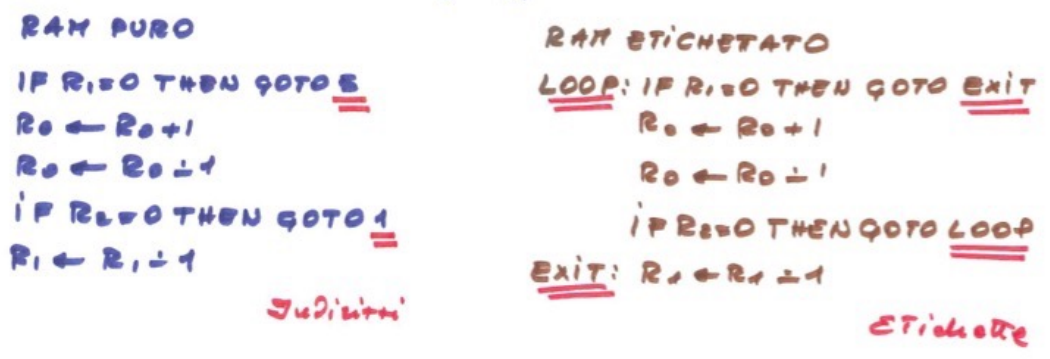
\includegraphics[scale=0.4]{images/ram_etichettato.png}
\end{figure}

semplicemente al posto di utilizzare i riferimenti numerici alle righe utilizzeremo delle parole,
con un semplice post-processing posso trasformare il "RAM etichettato" in "RAM puro" (l'aggiunta
di etichette non aumenta la potenza del linguaggio RAM).

\paragraph{Forma del compilatore}\mbox{}\\
Teniamo conto della natura degli oggetti su cui agirà il compilatore $W-PROG$ è un insieme definito
induttivamente. Questo significa che anche $Comp$ può essere definito induttivamente.

\begin{enumerate}
    \item mostriamo come compilare le basi di quel linguaggio, quindi gli assegnamenti (base).
    \item posso usare l'ipotesi induttiva, quindi assumo di saper compilare il comando $Comp(C_1),\dots,Comp(C_m)$ e ti
          faccio vedere come compilare il comando composto
          $$\underline{\text{begin}}\;C_1;\dots ;C_m; \underline{\text{end}}$$
    \item posso usare l'ipotesi induttiva, quindi di saper compilare $Comp(C)$ e mostrarlo come compilare il comando
          $while$ che ha come corpo $C$, $\underline{\text{while}}\;x_n\neq 0\;\underline{\text{do}}\;C$
\end{enumerate}

In tale maniera si saprà come compilare tutto $W-PROG$. Sia nota la seguente proprietà di compilazione,
ogni volta che durante una traduzione incontreremo nel programma una variabile $x_k$ ad essa verrà
associata il registro $R_k$ (abbiamo tranquillamente lo spazio per mappare tutte le variabili, visto
che il numero di registri è infinito).

\paragraph{Base: assegnamenti}\mbox{}\\
Vogliamo considerare i seguenti frammenti RAM per eseguire gli assegnamenti base dei programmi WHILE:
\begin{itemize}
    \item $Comp(x_k:=0)=$
          \begin{figure}[H]
              \centering
              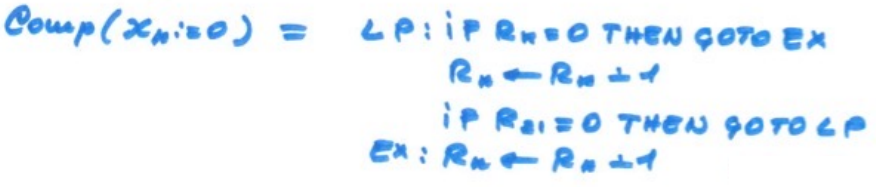
\includegraphics[scale=0.4]{images/assegnamento_ram.png}
          \end{figure}
          controllo se un registro è azzerato, nel caso non fosse azzerato allora lo decremento
          e ripeto il controllo ($R_21$ non sarà mai azzerato). Ad un certo punto uscirò dal ciclo,
          l'ultima operazione è praticamente nulla perché non danneggia l'operato precedente (è già zero).
          Tutti i registri da $R_21$ in poi sono tutti azzerati, perché non vengono utilizzati dal programma
          WHILE, quindi possiamo utilizzarli come meglio crediamo.

    \item $Comp(x_k:=x_j\pm 1)=$

          notiamo che c'è un caso dove la compilazione è immediata, in un caso di quest'istruzione
          troviamo subito l'istruzione RAM che fa la stessa cosa. Il caso particolare accade quando
          $k=j$. Se $k==j\rightarrow R_k\leftarrow R_k\pm 1$, il problema allora è nell'altro caso,
          ovvero quando $k\neq j$.

          \begin{figure}[H]
              \centering
              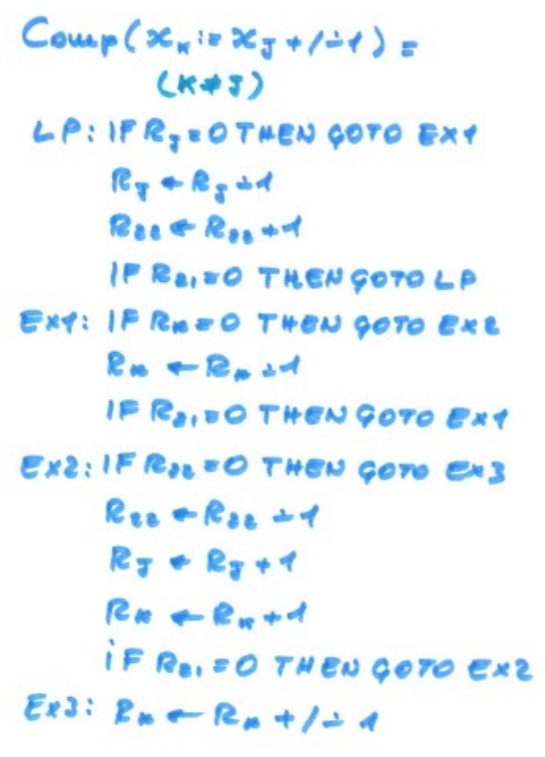
\includegraphics[scale=0.5]{images/assegnamento_ram2.png}
          \end{figure}
          \begin{enumerate}
              \item Salvo $x_j$ in $R_{22}$
              \item Azzero $x_k$, ovvero $R_k$
              \item Rigenero $x_j$ e $x_k$ da $R_{22}$
              \item Sommo/sottraggo 1 da $x_k$
          \end{enumerate}

          \paragraph{Passo induttivo}
          Consideriamo il comando composto $\underline{\text{begin}}\;C_1;...;C_m;\;\underline{\text{end}}$,
          considerando che esiste l'ipotesi induttiva, quindi assumo noti $Comp(C_1),\dots ,Comp(C_m)$
          mostro che la compilazione $Comp(\underline{\text{begin}}\;C_1;\dots;C_m\;\underline{\text{end}})$
          sarà:
          $$Comp(C_1);$$
          $$Comp(C_2);$$
          $$\dots$$
          $$Comp(C_m);$$

          Consideriamo il comando $\underline{\text{while}}\;x_k\neq 0\;\underline{\text{do}}\; C$,
          allora vogliamo mostrare che la compilazione $Comp(\underline{\text{while}}\;x_k\neq 0\;\underline{\text{do}}\; C)$
          corrisponde al frammento RAM:
          \begin{figure}[H]
              \centering
              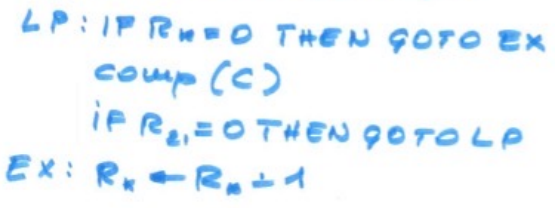
\includegraphics[scale=0.5]{images/comandowhile_ram.png}
          \end{figure}

          \paragraph{Ricapitolando}\mbox{}\\
          La funzione $Comp:W-PROG\rightarrow PROG$ che abbiamo definito induttivamente soddisfa:
          \begin{enumerate}
              \item è facilmente \textbf{programmabile}.
              \item compila ogni sorgente WHILE (\textbf{completo}).
              \item mantiene la semantica $\Psi_w=\varphi_{Comp(w)}\implies\textbf{ corretta}$
          \end{enumerate}
          I punti 2 e 3 si dimostrano facilmente per induzione strutturale, quindi possiamo dimostrare
          che $Comp$ è una traduzione da WHILE a RAM, e che quindi $F(WHILE)\subseteq F(RAM)$

\end{itemize}

\subsubsection{Dimostrazione $F(RAM)\subseteq F(WHILE)$}
Il problema in questo caso è dato dal fatto che di deve gestire il "go to", che non
è presente nel linguaggio WHILE (ed è proprio per questo motivo che utilizzare
goto nei linguaggi strutturati è solo un problema). Dimostreremo come è possibile evitare l'utilizzo
delle istruzioni "go to" nella programmazione strutturata.

Introduciamo il concetto di \textbf{interprete}, per quasi tutti i linguaggi di programmazione
ormai c'è la possibilità di avere la versione compilata che interpretata
(con differenze prestazionali).
La compilazione produce un programma equivalente che sta in piedi da solo
che può essere eseguito direttamente dalla macchina, l'interpretazione simula l'esecuzione
di un programma attraverso un interprete.

Vediamo come scrivere un interprete di programmi RAM scritto in WHILE, che chiameremo $I_W$.

\begin{figure}[H]
    \centering
    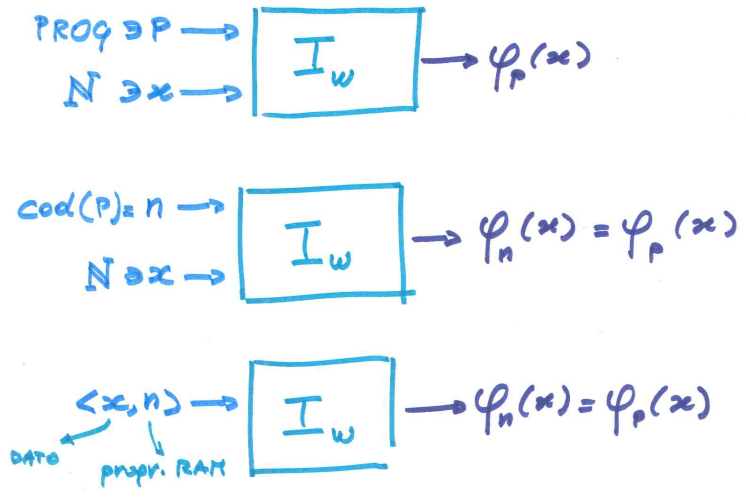
\includegraphics[scale=0.5]{images/interprete_while.png}
\end{figure}
Esso prenderà in ingresso un programma scritto in RAM ed un input, e produrrà in uscita
non un codice oggetto ma la semantica del programma $P$ sul dato $x$. Notiamo che in ingresso
viene dato un programma $P$ che è listato, ma sappiamo che i nostri programmi WHILE non lavorano
sulle stringhe. Un programma WHILE ha una sola variabile di input $x_1$ che può solo contenere
numeri.\textit{Come facciamo a fornire il listato di $P$ al programma WHILE?} Il mio $I_W$
prenderà in ingresso la codifica del programma $p$ che sarà fornito sotto forma di numero.

\textit{Ma il nostro programma può veramente prendere due dati in questa maniera?} Notiamo bene
che nel linguaggio WHILE $x_1$ non può prendere una coppia di numeri distinti, ma allora
dobbiamo passare un ulteriore coppia di Cantor di questi due numeri.

Il risultato sarà il funzionamento del programma con codice $n$ che in realtà è $P$.

Quindi la semantica di $I_W$:
$$\forall x,n\in\mathbb{N}:\Psi_{I_W}(\langle x,n\rangle)=\varphi_n(x)=\varphi_P(x)$$

\paragraph{Macro-WHILE}\mbox{}\\
Siccome devo scrivere un interprete in WHILE, voglio facilitarmi il lavoro utilizzando una
versione modificata del linguaggio (sempre permettendo di tornare al WHILE puro e senza
avere guadagni o perdite prestazionali). Questo per permettere di scrivere un codice
più semplice.

Per esempio:
\begin{figure}[H]
    \centering
    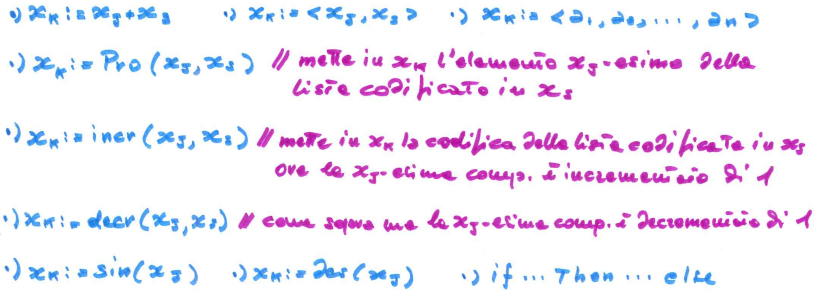
\includegraphics[scale=0.5]{images/macro-while.png}
\end{figure}

Come vediamo queste non sono istruzioni di WHILE puro, dovremmo scrivere molte più istruzioni
per ottenere ciò. Si ha anche la possibilità di rappresentare la coppia di cantor di due numeri,
visto che si ottengono con somme/sottrazioni, ed anche la possibilità di rappresentare la
lista di Cantor.

Ciascuna di queste MACRO può essere sostituita da un frammento di WHILE puro (seppur risulti piò comodo
da utilizzare)
$$F(MACRO-WHILE)=F(WHILE)$$




%\subsubsection{Forma del compilatore}
%$$comp:w-PROG\rightarrow PROG$$
%$w-PROG$ è un insieme costruito induttivamente, quindi $comp$ può essere definito induttivamente:
%\begin{enumerate}
%\item Mostrando come compilare le basi del linguaggio ovvero gli \textit{assegnamenti} (base).
%\item Per ipotesi induttiva assumo di saper compilare i seguenti comandi
%$$Comp(C_1),...,Comp(C_m)$$
%e mostrare come compilare il comando composto
%$\underline{\text{begin}}\;C_1; ...; C_m;\underline{\text{end}}$
%\item Per ipotesi induttiva di saper compilare il comando $Comp(C)$ e mostrare come
%compilare il comando while che ha come corpo $C$ $\text{while }x_n\neq 0 \text{ do } C$
%\end{enumerate}

%Adesso vediamo nello specifico come compilare ciascuno di questi punti



%lez 8
%Vogliamo dimostrare che la potenza computazionale della macchina RAM $F(RAM)$ sia disgiunto
%dalla potenza computazionale $F(WHILE)$.



\end{document}